% Created 2018-04-21 Sat 02:54
% Intended LaTeX compiler: pdflatex
\documentclass[bigger,unknownkeysallowed]{beamer}
\usepackage[utf8]{inputenc}
\usepackage[T1]{fontenc}
\usepackage{graphicx}
\usepackage{grffile}
\usepackage{longtable}
\usepackage{wrapfig}
\usepackage{rotating}
\usepackage[normalem]{ulem}
\usepackage{amsmath}
\usepackage{textcomp}
\usepackage{amssymb}
\usepackage{capt-of}
\usepackage{hyperref}
\usepackage{xcolor}
\usepackage{listings}
\titlegraphic{
\includegraphics{ccbysa.png}}
\lstset{escapeinside={'}{'},basicstyle=\scriptsize\ttfamily,showspace=false}
%\usepackage{ccicons}
\usetheme{ucadoc}
\author{Daniel Molina Cabrera}
\date{Curso de Python (Abril 2018)}
\title{Curso de Python: Nivel Inicial}
\hypersetup{
 pdfauthor={Daniel Molina Cabrera},
 pdftitle={Curso de Python: Nivel Inicial},
 pdfkeywords={},
 pdfsubject={},
 pdfcreator={Emacs 25.1.1 (Org mode 9.0.9)}, 
 pdflang={English}}
\begin{document}

\maketitle
\AtBeginSection[]{ \begin{frame}{Índice}     \tableofcontents[currentsection]     \end{frame} }
\section{}
\label{sec:org5288aef}
\begin{frame}
\frametitle{Contenido del tema}
\tableofcontents[hideallsubsections,part=1]
\end{frame}

\begin{frame}
\frametitle{Contenido del tema}
\tableofcontents[hideallsubsections,part=2]
\end{frame}




\begin{frame}[label={sec:orge018b29}]{Sobre mí}
\begin{columns}
\begin{column}{0.3\columnwidth}
\begin{center}

\includegraphics[width=\textwidth]{me.jpg}
\end{center}
\end{column}
\begin{column}{0.7\columnwidth}
\begin{block}{Sobre mí}
\begin{itemize}
\item Daniel Molina Cabrera.

\item Email: \href{mailto:dmolina@decsai.ugr.es}{dmolina@decsai.ugr.es}

\item Profesor de Informática en Ceuta-UGR.

\item Feliz programador de Python desde hace más de 15 años.

\item Desarrollador oficial de varios paquetes Python en Pypi.

\item Impartido varias asignaturas usando Python.

\item Defensor \emph{a ultranza} del software libre.
\end{itemize}


\part{1}
\end{block}
\end{column}
\end{columns}
\end{frame}
\section{Introducción sobre Python  ¿Por qué Python?}
\label{sec:orgfbaba3b}

\begin{frame}[label={sec:orgb89cb83}]{¿Qué es Python?}
\begin{center}
\includegraphics<1>[width=.4\textwidth]{python_real.jpg}
\includegraphics<2->[width=.4\textwidth]{monty_python.jpg}
\includegraphics<2->[width=.4\textwidth]{python_logo.png}
\end{center}

\pause
\pause

\begin{block}{Es un lenguaje de programación}
\begin{itemize}
\item Es un lenguaje para programar todo tipo de aplicaciones.

\item Se diseñó para que fuese \alert{fácil de usar} y \alert{divertido}.
\end{itemize}
\end{block}
\end{frame}


\begin{frame}[label={sec:org84a683a}]{¿Quién lo inventó?}
\begin{center}
\begin{center}

\includegraphics[width=0.5\textwidth]{PythonProgLogo.png}
\end{center}
\end{center}

\begin{columns}
\begin{column}{0.3\columnwidth}
\begin{center}
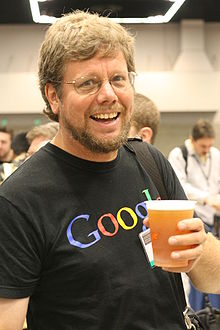
\includegraphics[width=\textwidth]{guido.jpg}
\end{center}
\end{column}

\begin{column}{0.8\columnwidth}
\begin{itemize}
\item Inventado por Guido Van Rossum.

\item Creado en 1989 en vacaciones de navidad.

\item Pensado para enseñar programación a niños.

\item Muy bien aceptado por la comunidad.

\item No dependiente del autor: dilema del autobús.

\item Influyente: Ruby, \ldots{}
\end{itemize}
\end{column}
\end{columns}
\end{frame}

\begin{frame}[label={sec:org5913aa9}]{¿Por qué Python? Es popular}
\begin{figure}[htbp]
\centering
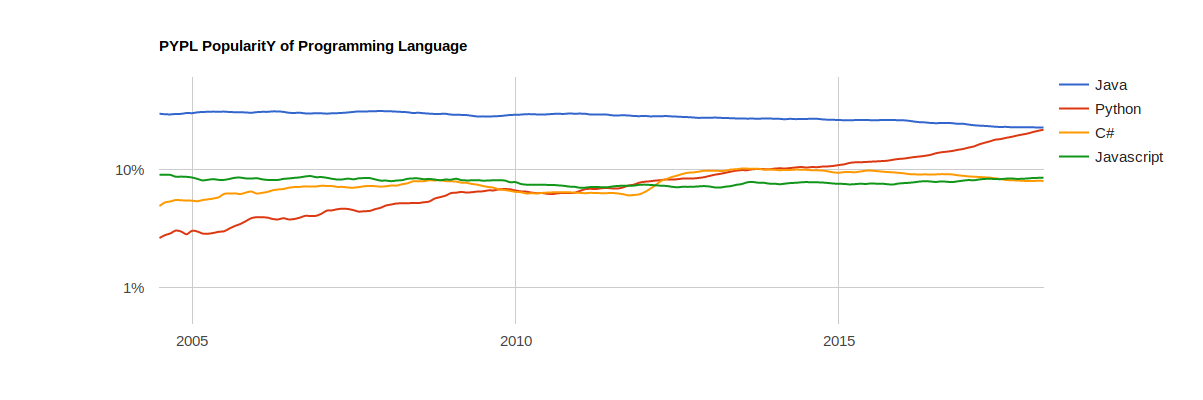
\includegraphics[width=\textwidth]{popularidad_tutoriales.png}
\caption{consulta de tutoriales (fuente: \href{https://pypl.github.io/PYPL.html}{PYPL (Google Trends)})}
\end{figure}

\begin{center}
{\Large {\color{blue}Es popular}}
\end{center}
\end{frame}

\begin{frame}[label={sec:orgfcafb43}]{¿Por qué Python? Es popular}
\begin{table}[htbp]
\caption{evolución  en TIOBE}
\centering
\begin{tabular}{rrlll}
\hline
Marzo 2018 & Marzo 2017 & Lenguaje & Porcentaje & Evolución\\
\hline
1 & 1 & Java & 14.941\% & -1.44\%\\
2 & 2 & C & 12.760\% & +5.02\%\\
3 & 3 & C++ & 6.452\% & +1.27\%\\
4 & 5 & Python & 5.869\% & +1.95\%\\
5 & 4 & C\# & 5.067\% & +0.66\%\\
\hline
\end{tabular}
\end{table}
\end{frame}


\begin{frame}[label={sec:org35a2060}]{Tengo unas gráficas más\footnote{source: \url{https://bit.ly/2f54vYk}\label{org464d895}}}
\begin{center}
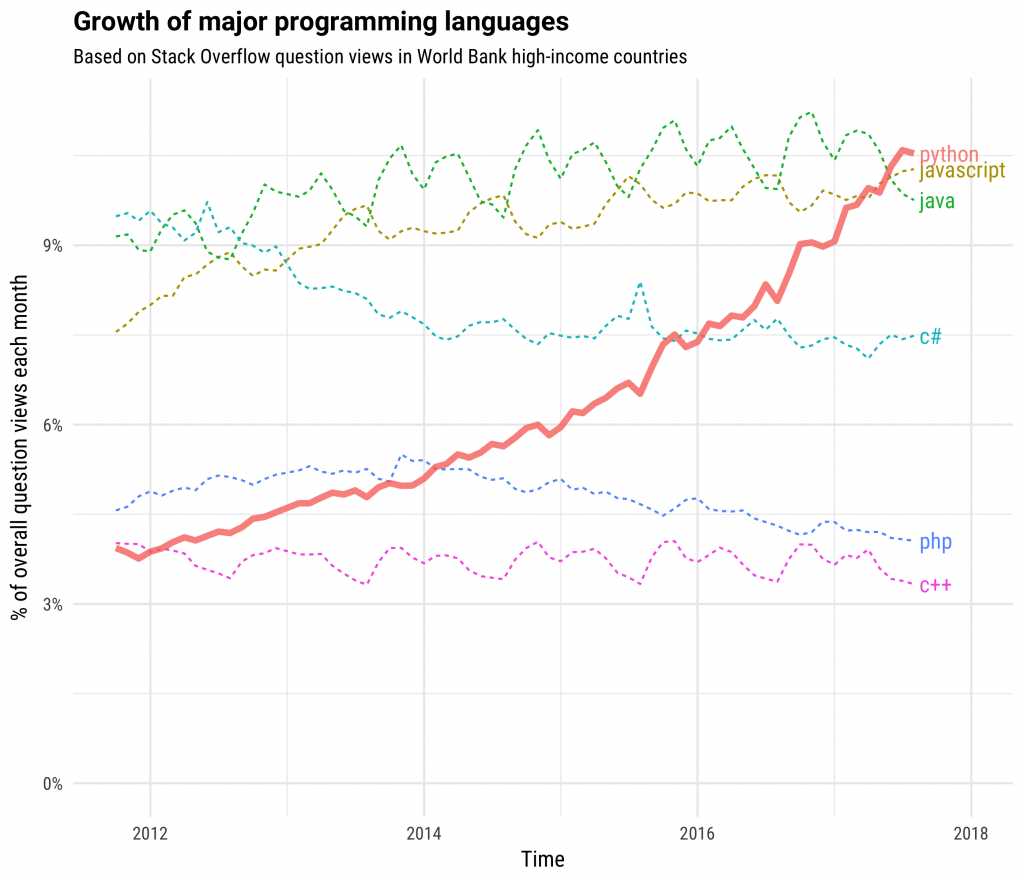
\includegraphics[height=.7\textheight]{growth.png}
\end{center}
\end{frame}

\begin{frame}[label={sec:org25c6815}]{Muchas más gráficas \textsuperscript{\ref{org464d895}}}
\begin{center}
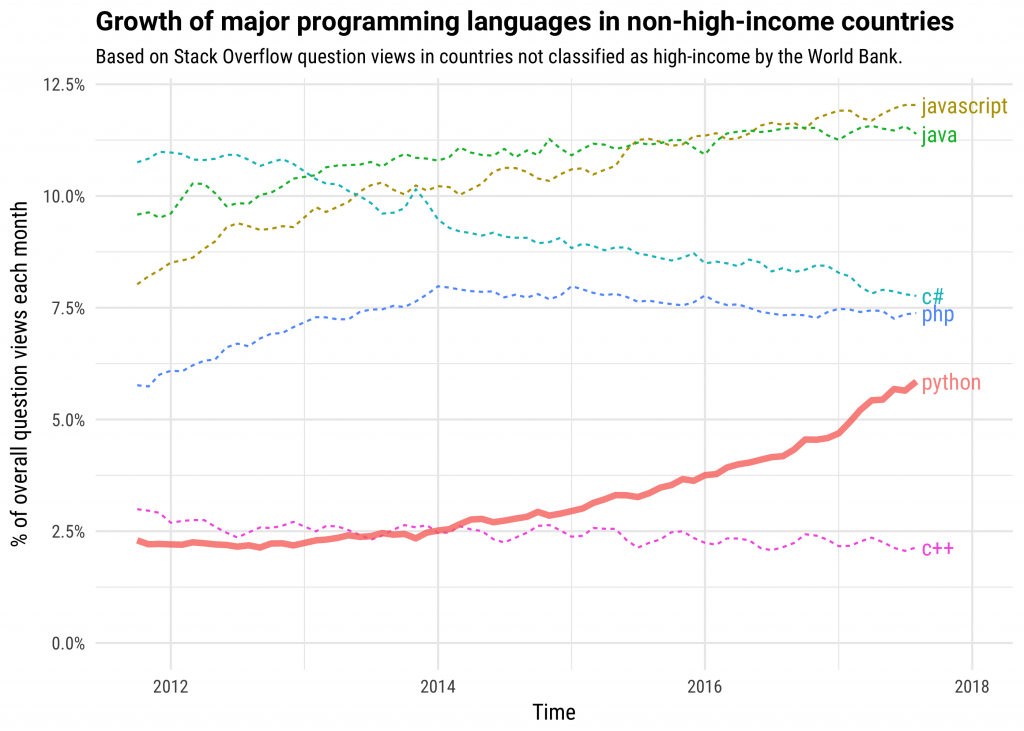
\includegraphics[height=.8\textheight]{non_hight.png}
\end{center}
\end{frame}

\begin{frame}[label={sec:orgd2da2cc}]{Visión general de crecimiento\textsuperscript{\ref{org464d895}}}
\begin{center}
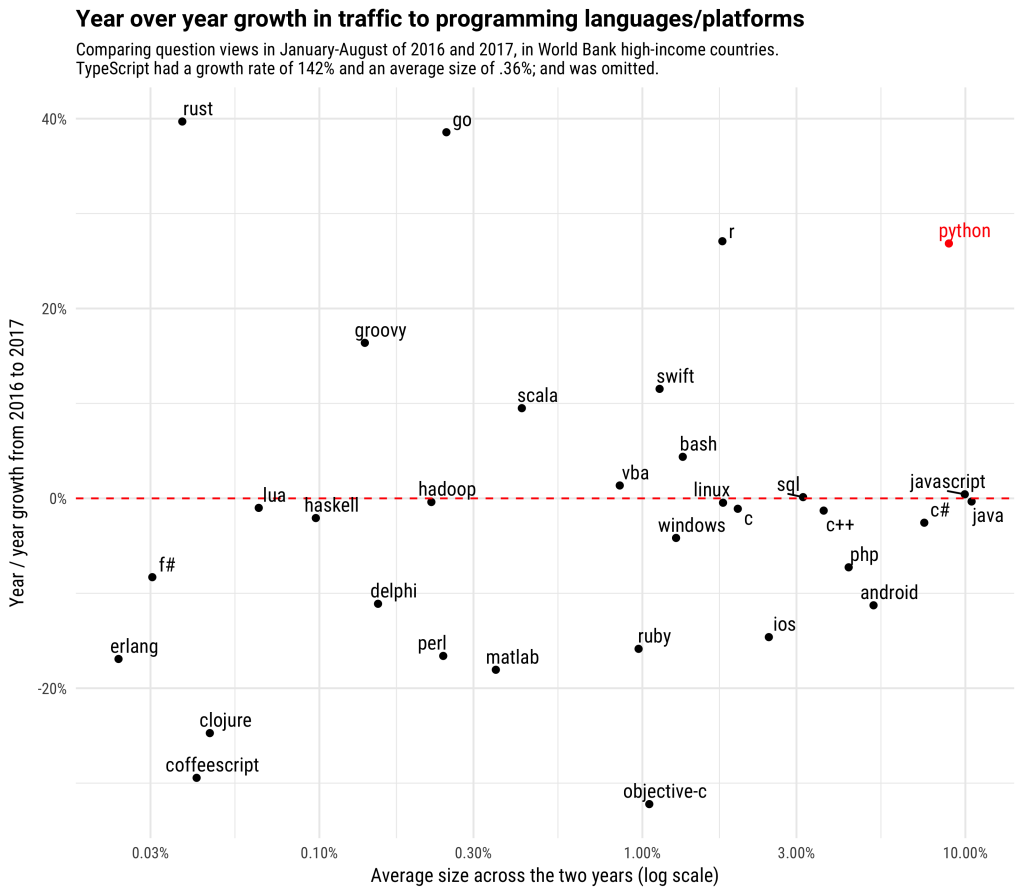
\includegraphics[height=.7\textheight]{tag_grown.png}
\end{center}
\end{frame}

\begin{frame}[label={sec:org0a174f7}]{¿Quién lo usa?}
\begin{center}

\includegraphics[width=\textwidth]{quienlousa.png}
\end{center}
\end{frame}

\begin{frame}[label={sec:org261f518}]{¿Y en temas actuales?}
\begin{center}
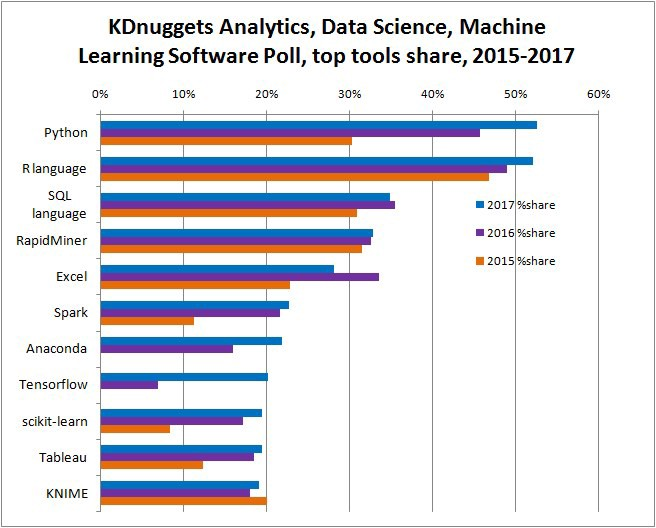
\includegraphics[height=\textheight]{python_machine_learning.png}
\end{center}
\end{frame}

\begin{frame}[label={sec:org7ea6c9e}]{Pero eso no es lo importante}
\begin{center}
\begin{center}

\includegraphics[width=\textwidth]{whyus.png}
\end{center}
\end{center}
\end{frame}

\begin{frame}[label={sec:org3cc30f7}]{Ventajas de Python: Portabilidad}
\begin{center}
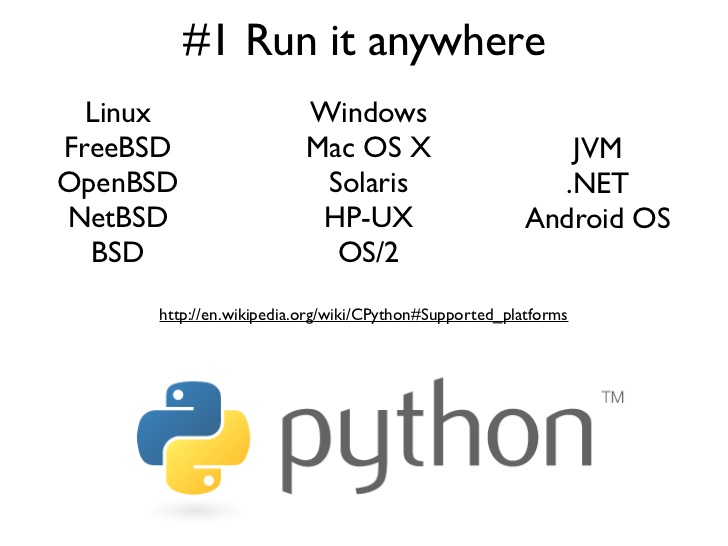
\includegraphics[width=\textwidth]{runanywhere.jpg}
\end{center}
\end{frame}


\begin{frame}[fragile,label={sec:orged132b1}]{Portabilidad}
 \begin{block}{Es un lenguaje interpretado}
\begin{itemize}
\item No se compila a ejecutable.

\item Se necesita Python para ejecutar.

\begin{itemize}
\item Disponible en distintos sistemas operativos.
\end{itemize}
\end{itemize}
\end{block}

\begin{block}{Ejemplo de uso}
\begin{verbatim}
python hello.py
\end{verbatim}
\scriptsize
\end{block}
\begin{block}{Otra opción (Linux)}
\begin{verbatim}
#!/usr/bin/env python3
print("hola a todos")
\end{verbatim}

\begin{verbatim}
chmod a+x hello.py
./hello.py
\end{verbatim}
\scriptsize
\begin{verbatim}
mayor que 0
\end{verbatim}
\end{block}
\end{frame}

\begin{frame}[label={sec:org5270979}]{Ventajas de Python: Legibilidad}
\begin{center}

\includegraphics[width=0.8\textwidth]{easy.jpg}
\end{center}
\end{frame}


\begin{frame}[fragile,label={sec:org0a74128}]{Ventajas de Python: Legibilidad}
 \begin{block}{C/C++}
\begin{verbatim}
#include <iostream>

int main(void) {
  std::cout <<"Hola a todos desde C++" <<std::endl;
}
\end{verbatim}
\end{block}

\begin{block}{Java}
\begin{verbatim}
class Main {
    public static void main(String[] args) {
	System.out.println("Hola a  todos desde Java");
    }
}
\end{verbatim}
\end{block}

\begin{block}{Python}
\begin{verbatim}
print("Hola a todos desde Python\n")
\end{verbatim}
\end{block}
\end{frame}

\begin{frame}[fragile,label={sec:orgfaa25ae}]{Ventajas de Python: Legibilidad, Alto nivel}
 \begin{exampleblock}{Admite variables alto nivel}
\begin{verbatim}
list = ["fruta", "cereales", "berenjena"]

for item in list:
    print(item)
\end{verbatim}
\end{exampleblock}

\begin{exampleblock}{Ejemplo: Implementar programa grep}
\begin{verbatim}
from sys import argv

def main(fname, word):
    with open(fname, "r") as file:
	for line in file:
	    if word in line:
		print(line)


if __name__ == "__main__":
    main(argv[2], argv[1])
\end{verbatim}
\end{exampleblock}
\end{frame}


\begin{frame}[label={sec:org716d4af}]{Ventajas de Python: Legibilidad, Alto nivel}
\begin{center}

\includegraphics[width=0.8\textwidth]{pseudo.jpg}
\end{center}
\end{frame}


\begin{frame}[label={sec:org15e02b8}]{El Zen de Python}
\begin{block}{Zen de Python, de Tim Peters}
\begin{verse}
Beautiful is better than ugly.\\
Explicit is better than implicit.\\
Simple is better than complex.\\
Complex is better than complicated.\\
Flat is better than nested.\\
Sparse is better than dense.\\
Readability counts.\\
\end{verse}
\end{block}

\begin{block}{Criterios de diseño de Python}
\begin{itemize}
\item Diseñado para simplicidad.
\end{itemize}
\end{block}
\end{frame}

\begin{frame}[label={sec:orgd4f30ec}]{Ventajas de Python: Comunidad}
\begin{block}{Lenguaje \emph{open source}}
\begin{itemize}
\item Dirigido por la comunidad.
\item \href{https://github.com/vinta/awesome-python}{Todo tipo de librerías}.
\item Repositorio de librerías disponibles.
\end{itemize}
\end{block}

\begin{block}{Versátil}
\begin{description}
\item[{Aplicaciones escritorio}] PyQt, \ldots{}.
\item[{automatización}] Fabric, celery, \ldots{}
\item[{Aplicaciones webs}] Django, Flask.
\item[{Software científico}] Numpy, Pandas, Matplotlib.
\item[{Machine Learning}] NLTK, TensorFlow, Scikit-learn.
\end{description}
\end{block}
\end{frame}


\begin{frame}[label={sec:org3881acb}]{Ventajas de Python: Comunidad}
\begin{figure}[htbp]
\centering
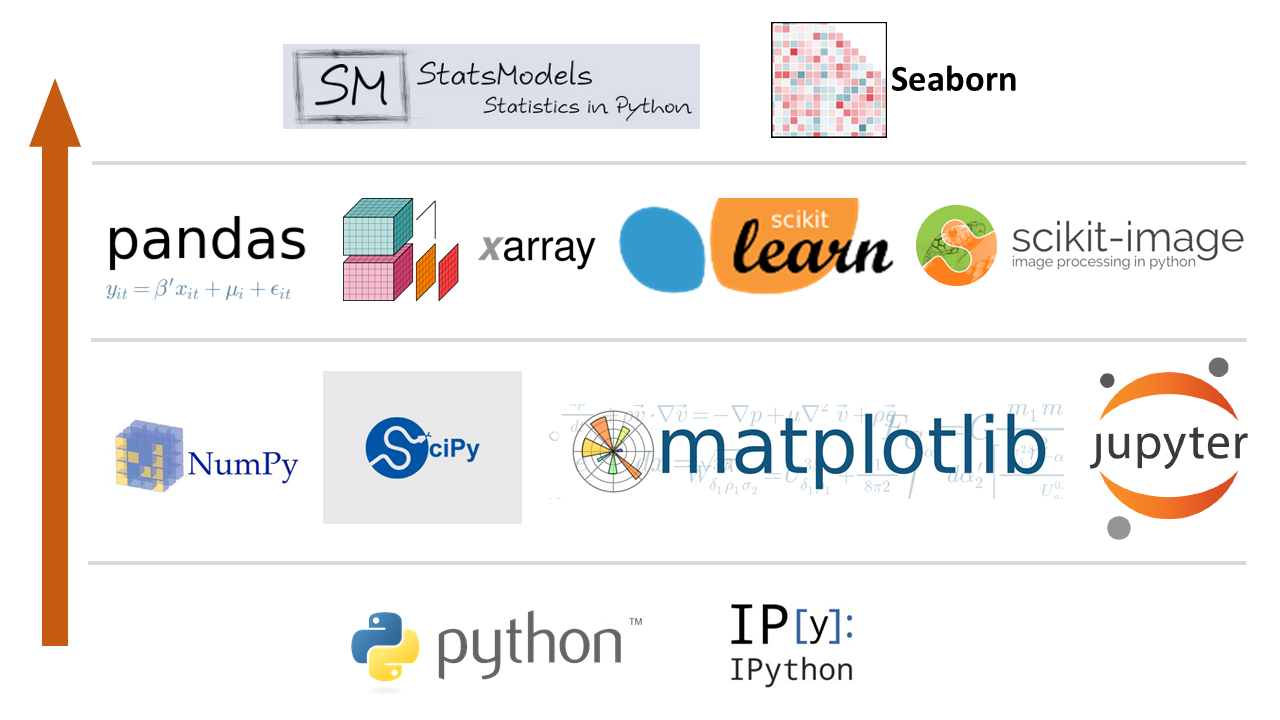
\includegraphics[width=0.8\textwidth]{librerias_ciencia.png}
\caption{Librerías de software científico}
\end{figure}
\end{frame}

\begin{frame}[label={sec:org43895cc}]{Pero sobre todo}
\begin{columns}
\begin{column}{0.5\columnwidth}
\begin{center}
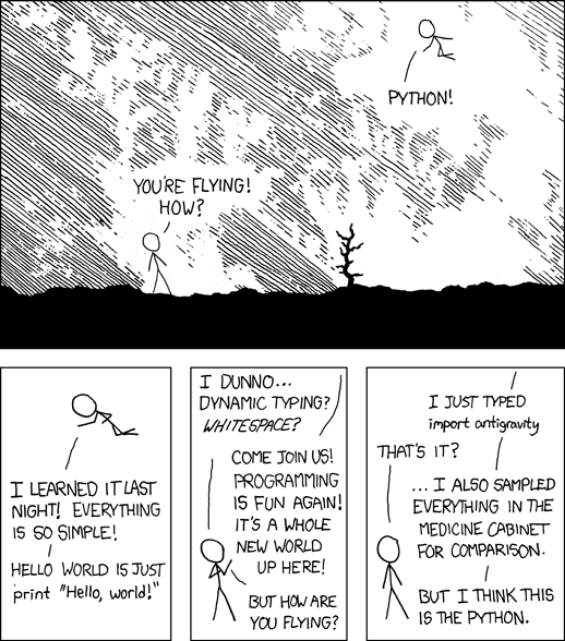
\includegraphics[width=.9\linewidth]{flying_joke.png}
\end{center}
\end{column}

\begin{column}{0.5\columnwidth}
\begin{center}

\includegraphics[width=.9\linewidth]{isfun.jpg}
\end{center}
\end{column}
\end{columns}
\end{frame}

\section{Sobre el curso}
\label{sec:org98aad8c}


\begin{frame}[label={sec:orge76284a}]{¿Qué necesito?}
\begin{columns}
\begin{column}{0.3\columnwidth}
\begin{center}
\begin{center}

\includegraphics[width=.8\textwidth]{python_logo.png}
\end{center}
\end{center}
\end{column}


\begin{column}{0.3\columnwidth}
\begin{center}
\begin{center}

\includegraphics[width=.8\textwidth]{logo-anaconda.png}
\end{center}
\end{center}
\end{column}
\begin{column}{0.3\columnwidth}
\begin{center}
\begin{center}

\includegraphics[width=\textwidth]{brain3.jpg}
\end{center}
\end{center}
\end{column}
\end{columns}

\begin{block}{Requisitos}
\begin{itemize}
\item Un ordenador.

\item Da igual el SO: Windows, Linux, MacOS.

\item Instalaremos Python3 usando Anaconda (opcional si ya está instalado).

\item Ocupa espacio, pasaré un \emph{pendrive}.
\end{itemize}
\end{block}
\end{frame}

\begin{frame}[label={sec:org0f1b801}]{¿Cómo será?}
\begin{center}
\begin{center}

\includegraphics[width=0.6\textwidth]{clase.png}
\end{center}
\end{center}

\begin{columns}
\begin{column}{0.5\columnwidth}
\begin{block}{Interactivo}
\begin{itemize}
\item Trabajaremos en Python.
\item Estilo taller.
\end{itemize}
\end{block}
\end{column}

\begin{column}{0.5\columnwidth}
\begin{block}{Sin conocimientos previos}
\begin{itemize}
\item De otros lenguajes.
\begin{itemize}
\item Siempre útil.
\end{itemize}

\item Estilo \emph{Pythonico}.
\end{itemize}
\end{block}
\end{column}
\end{columns}
\end{frame}

\begin{frame}[label={sec:orgf123b0e}]{¿Qué veremos?}
\begin{block}{Parte 1: Python y Sintaxis}
\begin{itemize}
\item Qué es y qué ofrece Python (Visto)

\item Instalación de Python y entornos.

\item Sintaxis de Python:

\begin{itemize}
\item Tipos de datos.

\item Condicionales y bloques.

\item Bucles.

\item Manejo de listas e iteradores.

\item Definiendo funciones y clases.

\item Instalando y usando librerías.

\item Trabajando con ficheros
\end{itemize}
\end{itemize}
\end{block}
\end{frame}

\begin{frame}[label={sec:org6bd9782}]{¿Qué veremos?}
\begin{block}{Parte 2: Uso de Python en distintos entornos}
\begin{itemize}
\item Python en ciencia.

\item Gráficos con Python.

\item Páginas web con Python.
\end{itemize}
\end{block}
\end{frame}

\begin{frame}[label={sec:org41331af}]{Bibliografía}
\begin{columns}
\begin{column}{0.5\columnwidth}
\begin{center}
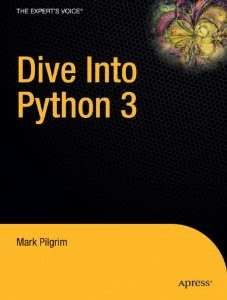
\includegraphics[width=0.5\textwidth]{cover_Driveinto3.jpg}
\end{center}
\end{column}

\begin{column}{0.5\columnwidth}
\begin{center}
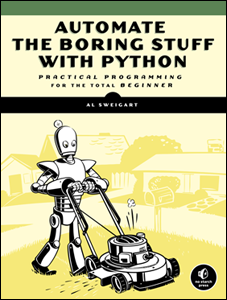
\includegraphics[width=0.5\textwidth]{cover_automate.png}
\end{center}
\end{column}
\end{columns}


\begin{block}{Referencias}
\begin{itemize}
\item \url{http://www.diveintopython.net/}
\item \url{https://automatetheboringstuff.com/}
\end{itemize}
\end{block}
\end{frame}

\section{Instalando Python y Entornos}
\label{sec:org9a7215a}

\begin{frame}[label={sec:org6b84d44}]{Instalando Python}
\begin{center}
\begin{center}

\includegraphics[width=.4\textwidth]{logo-anaconda.png}
\end{center}
\end{center}

\begin{block}{Instalación}
Disponible en \url{https://docs.anaconda.com/anaconda/install/}

\begin{itemize}
\item Windows.

\item Linux.

\item MacOS.
\end{itemize}
\end{block}
\end{frame}

\begin{frame}[label={sec:orgf06e69b}]{Instalando Python}
\begin{exampleblock}{En pendrive}
\begin{description}
\item[{Windows}] .exe (\url{https://www.anaconda.com/download/\#windows}).
\item[{Linux}] .sh (\url{https://www.anaconda.com/download/\#linux}).
\item[{MacOS}] .pkg (\url{https://www.anaconda.com/download/\#macos})
\end{description}
\end{exampleblock}
\end{frame}

\begin{frame}[label={sec:org3e6d6b4}]{Instalando en Windows}
\includegraphics<1>[width=.9\textwidth]{install_win1.png}
\includegraphics<2>[width=.9\textwidth]{install_win2.png}
\includegraphics<3>[width=.9\textwidth]{install_win3.png}
\includegraphics<4>[width=.9\textwidth]{install_win4.png}
\end{frame}

\begin{frame}[label={sec:orgf0a21a4}]{Instalando en MacOS}
\includegraphics<1>[width=.9\textwidth]{install_mac1.png}
\includegraphics<2>[width=.9\textwidth]{install_mac2.png}
\includegraphics<3>[width=.9\textwidth]{install_mac3.png}
\includegraphics<4>[width=.9\textwidth]{install_mac4.png}
\end{frame}

\begin{frame}[fragile,label={sec:org1cff257}]{Instalando en Linux}
 \begin{block}{Usando Anaconda}
\begin{verbatim}
bash ~/Downloads/Anaconda3-5.1.0-Linux-x86_64.sh
\end{verbatim}
\end{block}

\begin{block}{Desde el sistema de paquetes}
\begin{verbatim}
sudo apt install python3
python3 -m pip install --upgrade pip
python3 -m pip install jupyter
\end{verbatim}
\end{block}
\end{frame}

\begin{frame}[label={sec:orgc547380}]{Entornos}
\begin{block}{Formato interactivo}
\begin{description}
\item[{python}] Línea de forma interativa.
\item[{ipython/jupyer}] interfaz con \emph{esteroides} (autocompletado, \ldots{}).

\item[{ipython/jupyter notebook}] Interfaz web.
\end{description}
\end{block}

\begin{exampleblock}{Notebook}
\begin{itemize}
\item Entorno desde el navegador.

\item Fácil para pruebas rápidas (usaremos los primeros días).

\item Formato de ficheros \emph{.ipyb} aceptado por Github.
\end{itemize}
\end{exampleblock}

\begin{block}{Editores Específicos de Python}
\begin{description}
\item[{\href{http://thonny.org/}{Tonny}}] Editor para aprendizaje.

\item[{Spyder}] Disponible en Anaconda, integrado con consola.
\end{description}
\end{block}
\end{frame}

\begin{frame}[label={sec:org167c2dd}]{Ejemplo de entornos (Python por defecto)}
\begin{figure}[htbp]
\centering
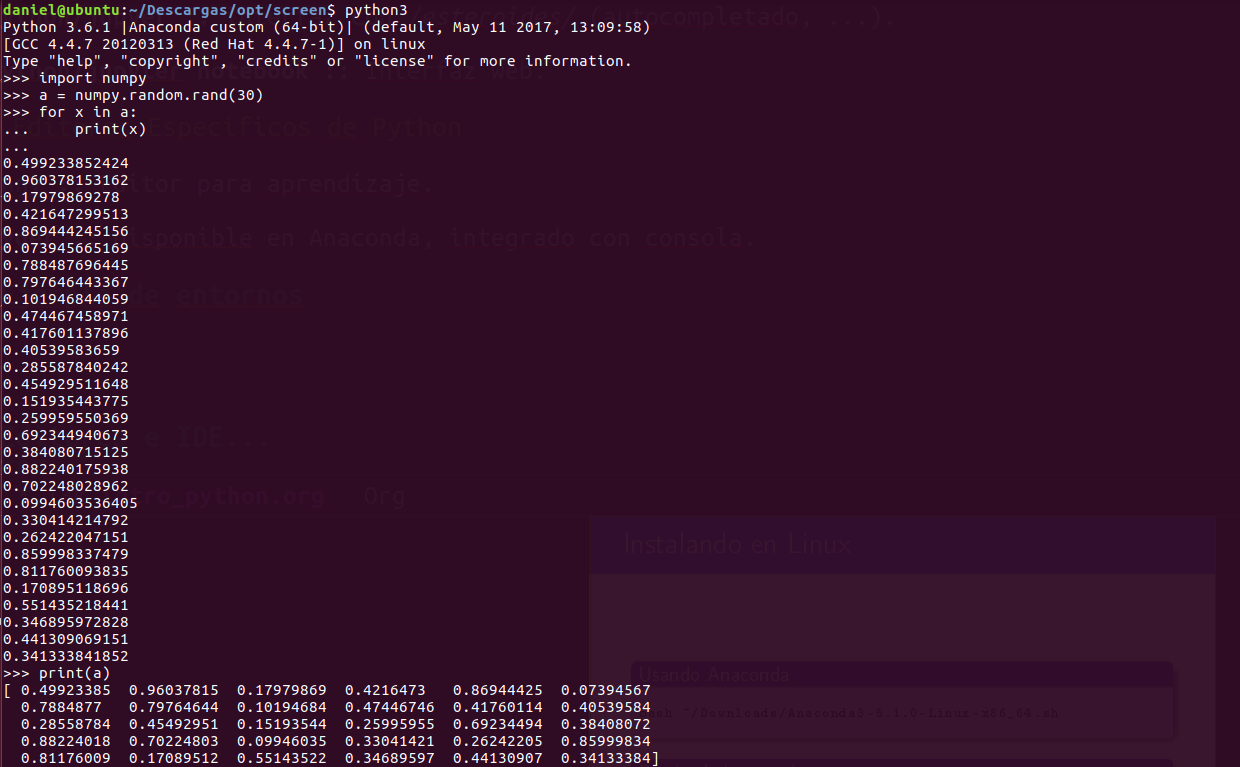
\includegraphics[width=.8\textwidth]{python.png}
\caption{consola por defecto de python}
\end{figure}
\end{frame}

\begin{frame}[label={sec:org451f506}]{Ejemplo de entornos (IPython/Jupyter)}
\begin{figure}[htbp]
\centering
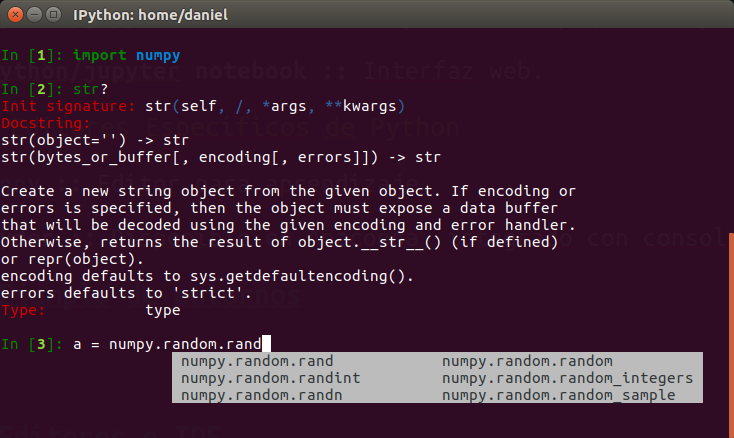
\includegraphics[width=.8\textwidth]{ipython.png}
\caption{consola de ipython/jupyter}
\end{figure}
\end{frame}

\begin{frame}[label={sec:org211832c}]{Ejemplo de entornos (IPython/Jupyter notebook)}
\begin{center}
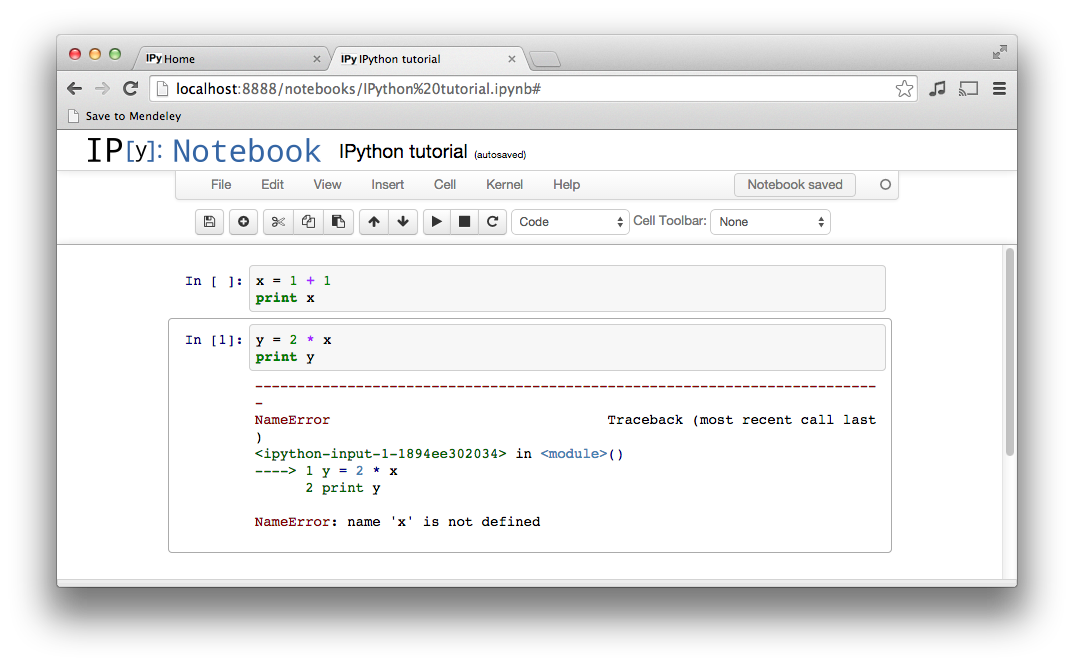
\includegraphics[width=.8\textwidth]{notebook1.png}
\end{center}
\end{frame}

\begin{frame}[label={sec:org89aa04c}]{Ejemplo de entornos (IPython/Jupyter notebook)}
\begin{center}
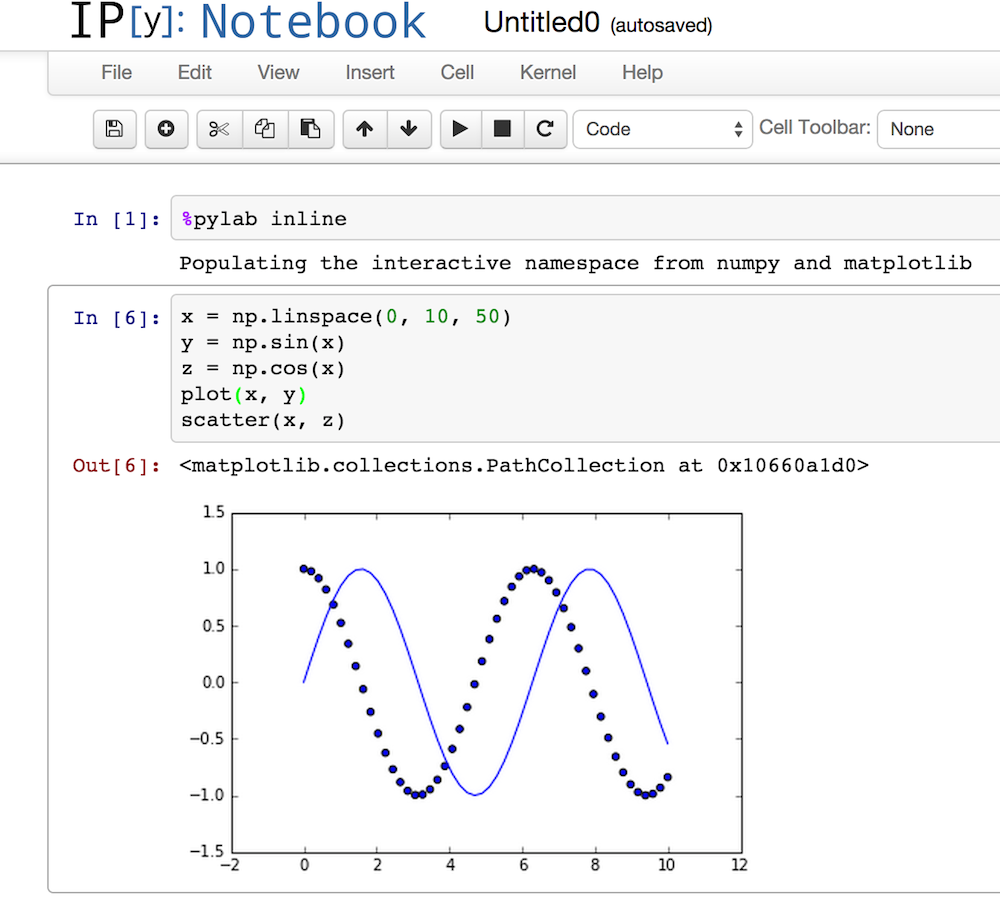
\includegraphics[width=.8\textwidth]{notebook2.png}
\end{center}
\end{frame}


\begin{frame}[label={sec:orga8fc3de}]{Ejemplo de entornos (Tonny)}
\begin{center}
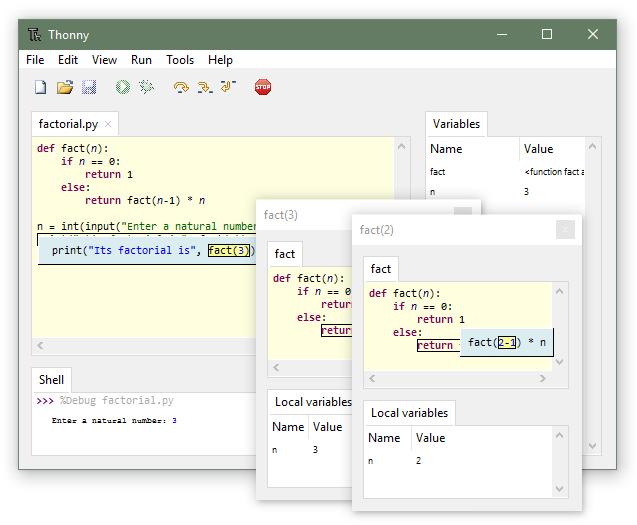
\includegraphics[width=.8\textwidth]{tonny.png}
\end{center}
\end{frame}

\begin{frame}[label={sec:orgb6d909f}]{Ejemplo de entornos (Spyder)}
\begin{center}
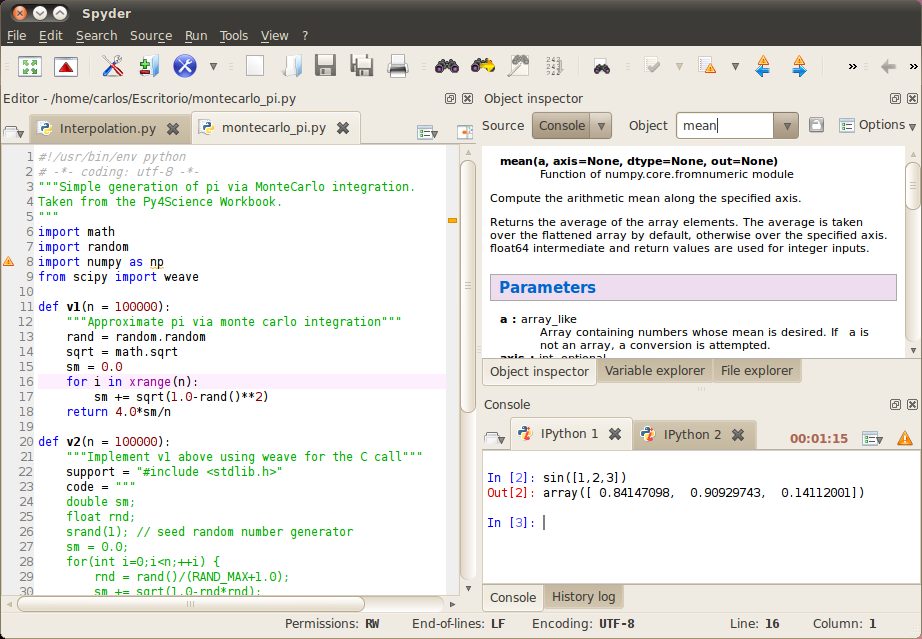
\includegraphics[width=.8\textwidth]{spyder.png}
\end{center}
\end{frame}



\begin{frame}[label={sec:orgb5d527d}]{Editores e IDE}
\begin{columns}
\begin{column}{0.32\columnwidth}
\begin{center}

\includegraphics[width=\textwidth]{atom_logo.png}
\end{center}
\end{column}

\begin{column}{0.2\columnwidth}
\begin{center}

\includegraphics[width=\textwidth]{sublimetext.png}
\end{center}
\end{column}

\begin{column}{0.2\columnwidth}
\begin{center}

\includegraphics[width=\textwidth]{neovim.png}
\end{center}
\end{column}

\begin{column}{0.15\columnwidth}
\begin{center}

\includegraphics[width=\textwidth]{spacemacs.png}
\end{center}
\end{column}
\end{columns}

\begin{block}{Editores Extensibles}
\begin{description}
\item[{Atom}] Editor de Github, muchos módulos.
\item[{SublimeText}] Editor no gratuito extensible, muy popular.
\item[{NeoVim}] Fork de vim.
\item[{Spacemacs}] Emacs preconfigurado.
\end{description}
\end{block}

\begin{block}{IDE completos}
\begin{description}
\item[{PyCharm}] Versión community, módulos de pago.
\item[{PyDev}] Módulo de eclipse.
\end{description}
\end{block}
\end{frame}


\begin{frame}[label={sec:org1b7c778}]{Ejemplo: PyCharm}
\begin{block}{Versiones}
\begin{itemize}
\item Community (y Educativa).
\item Comercial.
\end{itemize}
\end{block}

\begin{center}
\begin{center}
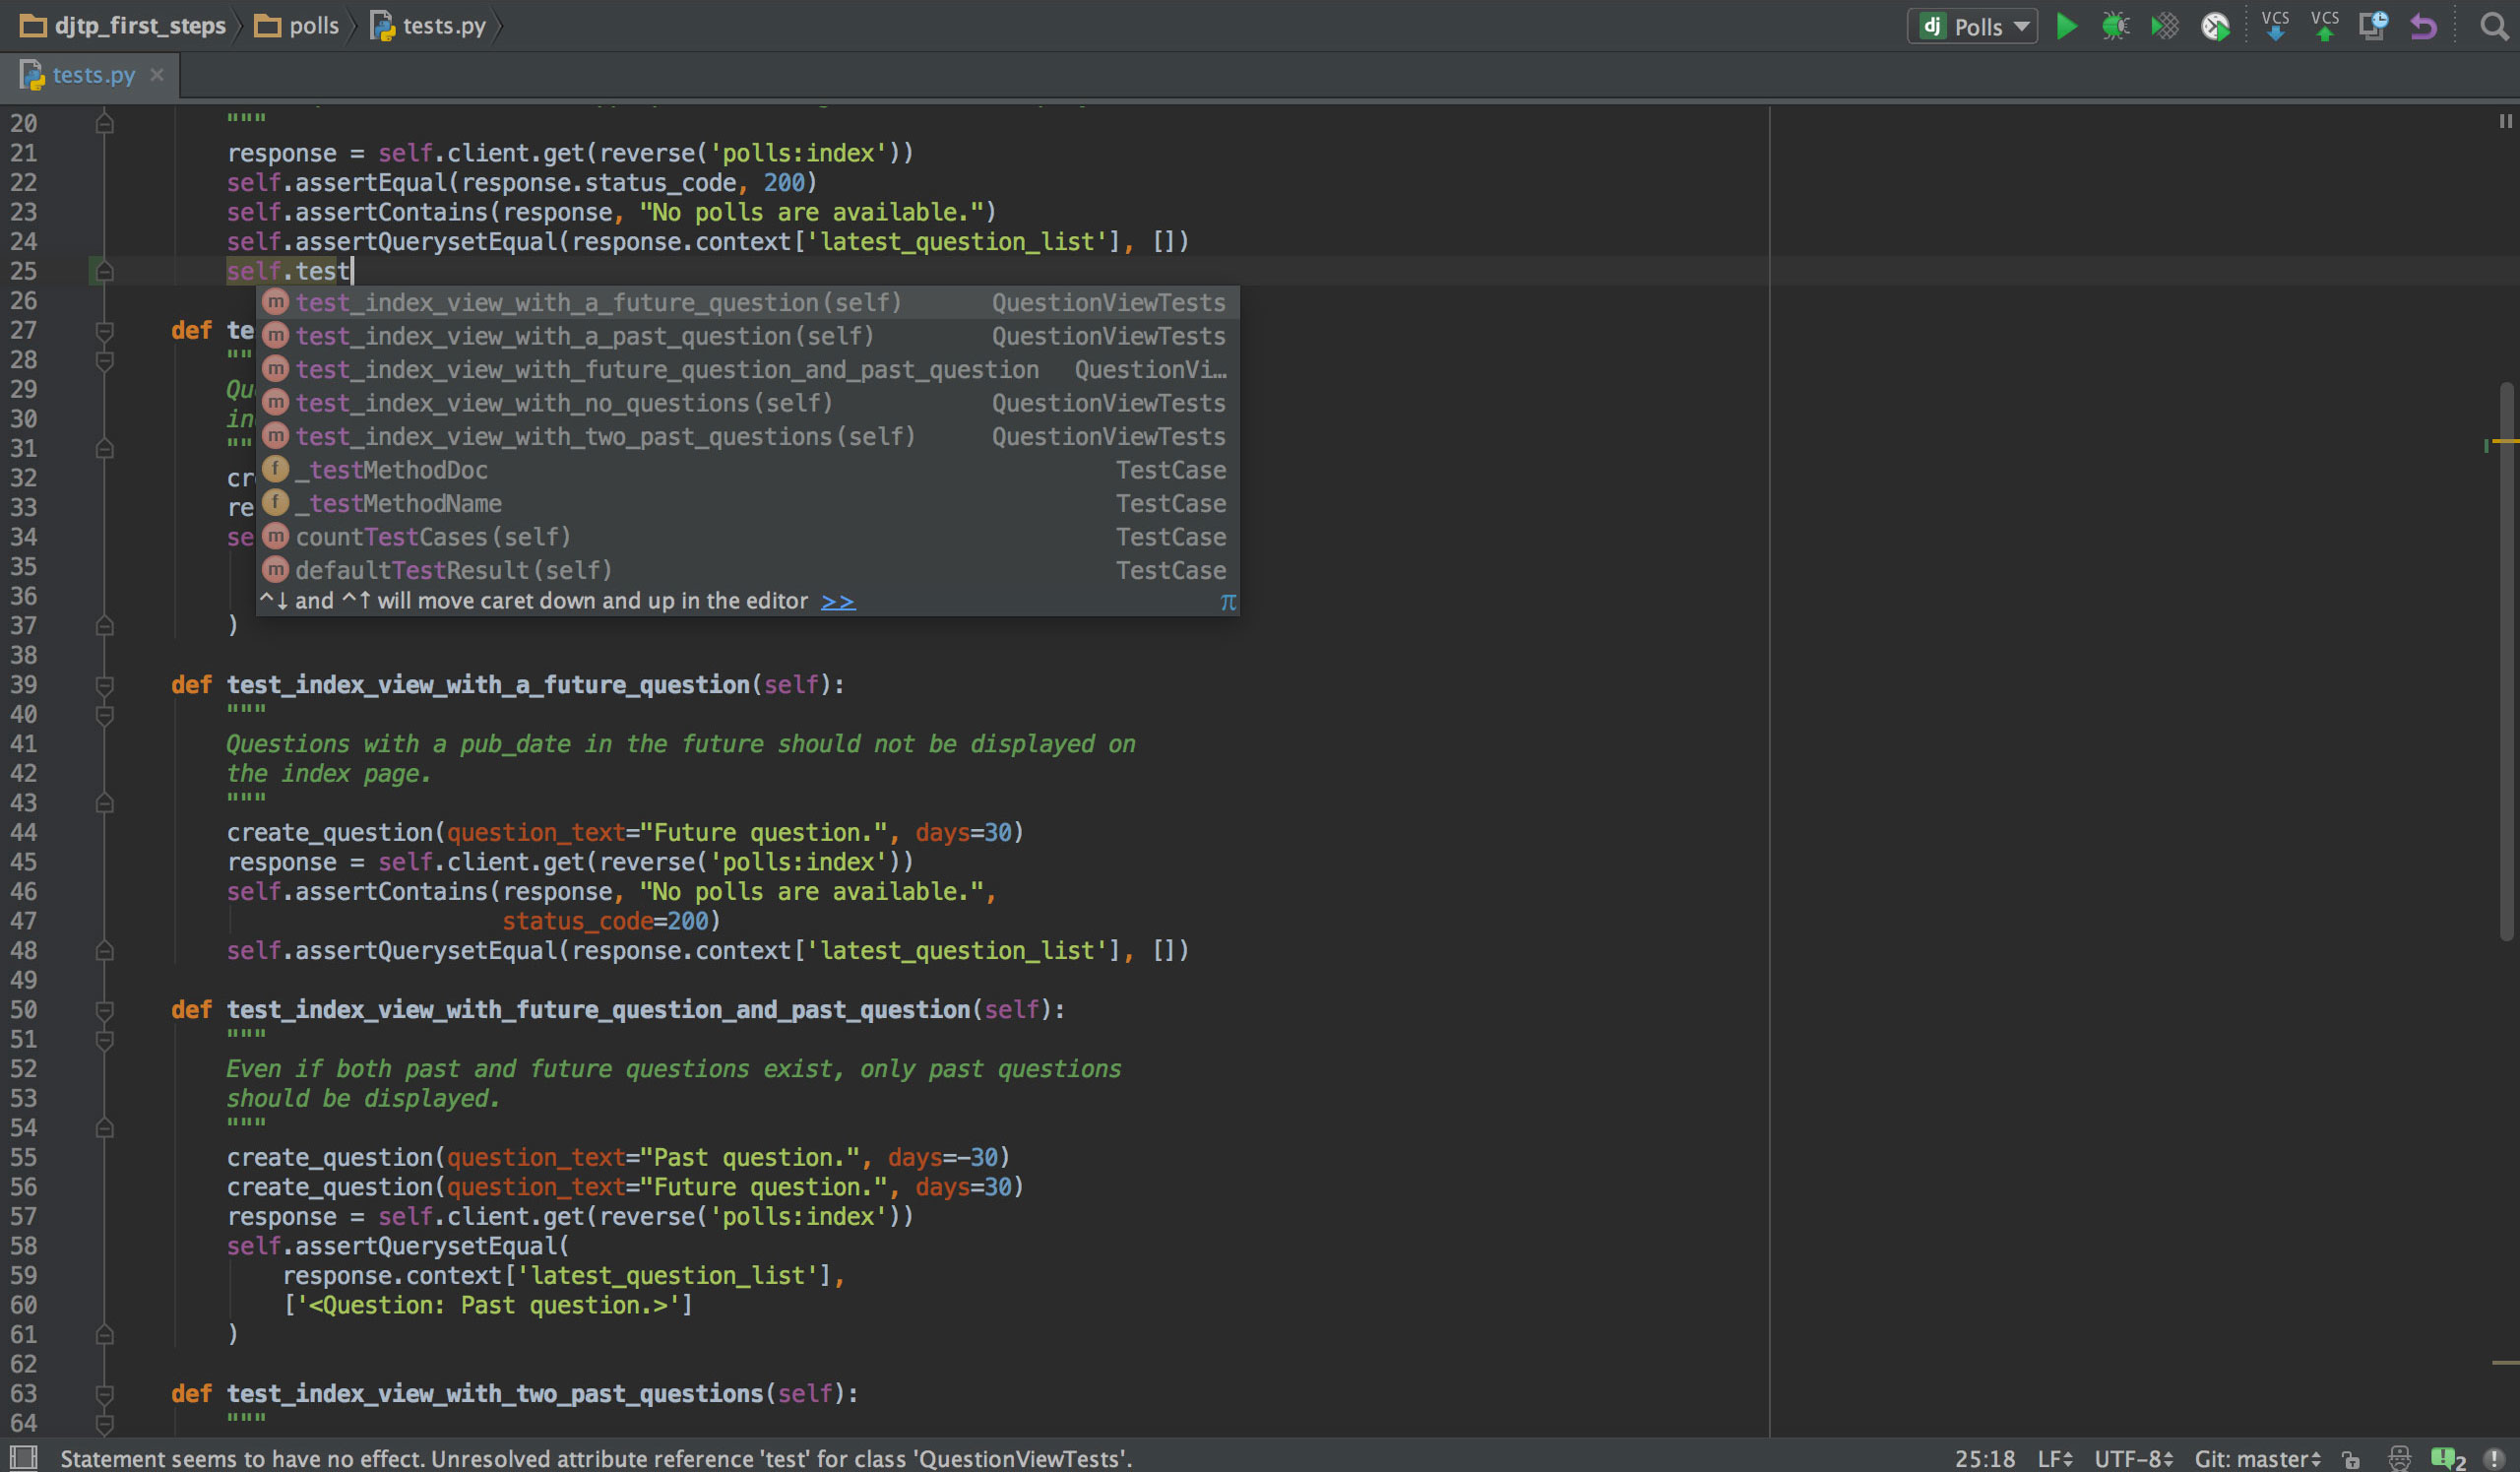
\includegraphics[width=.8\textwidth]{pycharm.png}
\end{center}
\end{center}
\end{frame}

\section{Empezando con Python}
\label{sec:orgc90a203}

\begin{frame}[label={sec:org19b7e98}]{Empezando con Python}
\begin{center}
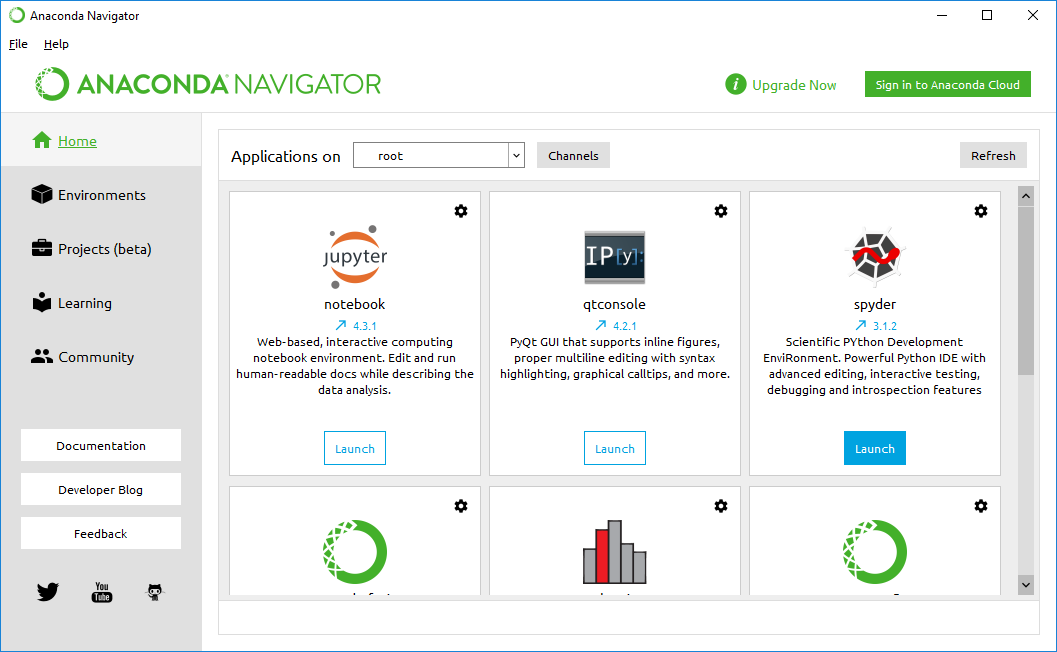
\includegraphics[width=.9\linewidth]{anaconda_navigator.png}
\end{center}

\begin{block}{Pasos}
\begin{enumerate}
\item Lanzar "Anaconda Navigator".

\item Seleccionar Jupyter Notebook.
\end{enumerate}
\end{block}
\end{frame}

\begin{frame}[fragile,label={sec:org98517c1}]{Variables}
 \begin{block}{}
\begin{verbatim}
msg = "Hola a todos"
print(msg)
\end{verbatim}
\begin{verbatim}
Hola a todos
\end{verbatim}

\begin{verbatim}
Hola a todos
\end{verbatim}
\end{block}

\begin{block}{Variables}
\begin{itemize}
\item Las variables permiten guardar datos.
\item Se accede a los valores usando el nombre de la variable.
\item Se puede modifican los valores durante la ejecución.
\end{itemize}
\end{block}

\begin{block}{}
\begin{verbatim}
a = 3
b = 4
print(a+b)
a = a+1
print(a+b)
\end{verbatim}
\scriptsize
\begin{verbatim}
7
8
\end{verbatim}
\end{block}
\end{frame}

\begin{frame}[fragile,label={sec:orgb6eefcf}]{Tipos de variables}
 \begin{block}{Las variables pueden guardar distinto tipo de datos}
\begin{description}
\item[{Números entero}] number = 3
\item[{Números real }] number\_real = 3.2
\item[{Cadena}] msg = "Hola"
\item[{Listas}] lista = [1, 2, 3]
\item[{Tabla hash}] datos = \{'c': "cerrar", 'd': "delete"\}
\end{description}
\end{block}

\begin{alertblock}{Diferencia}
\begin{itemize}
\item No hay que definir el tipo de una variable.
\item Una misma variable pueden tomar valores de distinto tipo (no recomendado).
\end{itemize}
\end{alertblock}

\begin{verbatim}
variable = 4
variable = "hola"
\end{verbatim}
\end{frame}

\begin{frame}[fragile,label={sec:org15c7a98}]{Ejemplo de uso}
 \begin{block}{Ejemplo de uso}
\begin{verbatim}
print(number+1)
print(number_real-1)
print(lista)
print(datos)
\end{verbatim}
\scriptsize
\begin{verbatim}
4
2.2
[1, 2, 3]
{'c': 'cerrar', 'd': 'delete'}
\end{verbatim}
\end{block}

\begin{alertblock}{Aviso}
Python tiene tipos, no se permiten operaciones entre tipos.
\end{alertblock}
\begin{block}{}
\begin{verbatim}
print(number+lista)
\end{verbatim}
\scriptsize
\begin{verbatim}
Traceback (most recent call last):
  File "<stdin>", line 1, in <module>
TypeError: unsupported operand type(s) for +: 'int' and 'list'
\end{verbatim}
\end{block}
\end{frame}


\begin{frame}[fragile,label={sec:orgdc32daa}]{Asignación de tipos en Python3}
 \begin{block}{En Python3 se incorporó definir tipos en variables}
\begin{verbatim}
count: int = 4
\end{verbatim}
\scriptsize
\end{block}
\begin{block}{Vamos a meter un error}
\begin{verbatim}
count: int = 4
count += 1.5
\end{verbatim}
\end{block}

\begin{alertblock}{El analizador (mypy) detecta errores en tipos}
\begin{verbatim}
python3 ej_typing.py
\end{verbatim}
\scriptsize
\begin{verbatim}
5.5
\end{verbatim}
\begin{verbatim}
python3 -m mypy ej_typing.py # or mpy ej_typing.py
\end{verbatim}
\scriptsize
ej\_typing.py:2: error: Incompatible types in assignment (expression has type "float", variable has type "int")
\end{alertblock}
\end{frame}

\begin{frame}[fragile,label={sec:org6ea0fcf}]{Usando variables}
 \begin{block}{Tipos entero}
\begin{verbatim}
number = 3
print(number+3)
print(number/2)
\end{verbatim}
\scriptsize
\begin{verbatim}
6
1.5
\end{verbatim}
\end{block}

\begin{alertblock}{División}
\begin{itemize}
\item Dividir números enteros devuelve un número real.
\item La división entera es otra operación: //.
\end{itemize}
\end{alertblock}

\begin{block}{}
\begin{verbatim}
number = 3
print(number//2)
\end{verbatim}
\scriptsize
\begin{verbatim}
1
\end{verbatim}
\end{block}
\end{frame}

\begin{frame}[fragile,label={sec:org91390ed}]{Usando variables}
 \begin{block}{Tipo real}
\begin{verbatim}
number = 3
number_real = number_real + number
print(number_real)
\end{verbatim}
\scriptsize
\begin{verbatim}
9.2
\end{verbatim}
\end{block}

\begin{block}{Tipo cadena}
\begin{verbatim}
msg = "hola"
print("a" in msg)
msg = msg + " adios"
print(msg)
\end{verbatim}
\scriptsize
\begin{verbatim}
True
hola adios
\end{verbatim}
\end{block}
\end{frame}

\begin{frame}[fragile,label={sec:orgb7bde27}]{Usando variables}
 \begin{block}{Tipo List}
\begin{verbatim}
lista2 = lista + [6]
print(lista)
print(lista2)
print(4 in lista)
print("El primer valor es ", lista2[0])
print("Los dos siguientes son", lista2[1:3])
print("Los siguientes son", lista2[1:])
\end{verbatim}
\scriptsize
\begin{verbatim}
[1, 2, 3]
[1, 2, 3, 6]
False
El primer valor es  1
Los dos siguientes son [2, 3]
Los siguientes son [2, 3, 6]
\end{verbatim}
\end{block}
\end{frame}

\begin{frame}[fragile,label={sec:org6c963d6}]{Bloques y Condicionales}
 \begin{block}{Condicionales}
\begin{itemize}
\item Aplicar el mismo código siempre igual no es \emph{divertido}.

\item Un programa puede ejecutar código según una condición.
\end{itemize}
\end{block}

\begin{exampleblock}{Ejemplo}
\begin{verbatim}
print("Dime un numero")
numero = int(input())

if numero == 7:
  print("Has acertado!!!\n")
else:
  print("Has fallado, mas suerte para otra\n")
\end{verbatim}
\end{exampleblock}
\end{frame}

\begin{frame}[fragile,label={sec:org082da0d}]{Bloques y condicionales}
 \begin{block}{Definiendo los bloques}
\begin{itemize}
\item Los bloques se marcan en otros lenguajes usando \{\ldots{}\}.

\item Por legibilidad se debe tabular.

\item Python se guía de la tabulación, es necesario un editor adecuado.
\end{itemize}
\end{block}

\begin{exampleblock}{Ejemplo}
\begin{verbatim}
cantidad = int(input())

if cantidad < 1000:
  if cantidad < 100:
    print("Eso es una miseria")
  else:
    print("Eso es poco")
else:
  print("Es mucho, pero te lo acepto por hacerte un favor")
\end{verbatim}
\end{exampleblock}
\end{frame}

\begin{frame}[fragile,label={sec:org0a78201}]{Condicionales}
 \begin{exampleblock}{Ejemplo}
\begin{verbatim}
if number > 5:
  print("mayor que 5")
\end{verbatim}
\end{exampleblock}

\begin{block}{Formato}
\begin{itemize}
\item Tras palabra \alert{if} se indica una condición y un \alert{:}.

\item El código tabulado se ejecuta sólo si la condición se cumple.

\item Puede ponerse un else, se ejecuta si no se cumple.
\end{itemize}
\end{block}

\begin{exampleblock}{Con else}
\begin{verbatim}
if number > 5:
  print("mayor que 5")
else:
  print("menor o igual que 5")
\end{verbatim}
\end{exampleblock}
\end{frame}

\begin{frame}[fragile,label={sec:org4fc366f}]{¿Y el switch?}
 \begin{block}{No tiene switch}
\begin{itemize}
\item Tiene muchas limitaciones en otros lenguajes.

\item tiene el \alert{elif}.
\end{itemize}
\end{block}

\begin{exampleblock}{Ejemplo}
\begin{verbatim}
if number > 0: 
  print("mayor que 0")
elif number > 5:
  print("mayor que 5")
else:
  print("menor o igual que 5")
\end{verbatim}
\end{exampleblock}
\end{frame}

\section{Listas}
\label{sec:org1e848d5}
\part{2}

\begin{frame}[fragile,label={sec:org5a22b64}]{Listas}
 \begin{block}{Listas}
\begin{itemize}
\item Permiten guardar varios valores en una variable.

\item Pueden ser de tipos distintos (no recomendable).
\item Se pueden acceder mediante corchetes y posición:
\begin{itemize}
\item 0 \(\Rightarrow\) primer elemento.
\item 1 \(\Rightarrow\) segundo elemento.
\item \ldots{}
\end{itemize}
\end{itemize}
\end{block}

\begin{block}{Ejemplos}
\begin{verbatim}
lista1 = ['monty', 'python', 42]
lista2 = [1, 2, 3, 4, 5]
print(lista1[1], lista1[2], lista2[3])
\end{verbatim}
\scriptsize
\begin{verbatim}
python 42 4
\end{verbatim}
\end{block}
\end{frame}

\begin{frame}[label={sec:org56d42db}]{Modificando elementos}
\begin{block}{Cambiando el valor}
\begin{description}
\item[{Directamente}] lista[ \emph{posicion} ] = \emph{nuevo valor}.
\end{description}
\end{block}

\begin{block}{Añadiendo elementos}
\begin{description}
\item[{Al final}] Método append (lo más eficiente).

\item[{Varios al final}] Operador + (ambos deben ser listas).

\item[{En medio}] Método insert (\emph{insert(posicion, valor)}).
\end{description}
\end{block}

\begin{block}{Borrando elementos}
\begin{description}
\item[{Todos los elementos}] Método clean.

\item[{Elemento concreto}] \emph{del lista[posicion]}.
\end{description}
\end{block}
\end{frame}
\begin{frame}[fragile,label={sec:org406bfdb}]{Modificando listas}
 \begin{columns}[t]
\begin{column}{0.5\columnwidth}
\begin{exampleblock}{Ejemplos}
\begin{verbatim}
lista = [1, 2, 3, 4, 5]
print(lista)
lista[2] *= 2
print(lista)
lista.append(9)
print(lista)
lista.insert(0, 0)
print(lista)
del lista[4]
print(lista)
lista = lista + [10, 11]
print(lista)
lista.clear()
print(lista)
\end{verbatim}
\end{exampleblock}
\end{column}

\begin{column}{0.5\columnwidth}
\begin{block}{Salida}
\scriptsize
\begin{verbatim}
[1, 2, 3, 4, 5]
[1, 2, 6, 4, 5]
[1, 2, 6, 4, 5, 9]
[0, 1, 2, 6, 4, 5, 9]
[0, 1, 2, 6, 5, 9]
[0, 1, 2, 6, 5, 9, 10, 11]
[]
\end{verbatim}
\end{block}
\end{column}
\end{columns}
\end{frame}


\begin{frame}[label={sec:org2d08081}]{Accediendo elementos}
\begin{block}{Accediendo elementos}
\begin{description}
\item[{Único elemento}] lista[ \emph{posicion} ]
\item[{Rango de elementos entre [inicio, fin[}] lista[ \emph{inicio}: \emph{fin} ]
\item[{Rango de elementos con salto}] lista[ \emph{inicio}: \emph{fin} : \emph{salto} ]
\item[{Rango antes de una posición}] lista[ : \emph{posicion} ]
\item[{Rango desde de una posición}] lista[ \emph{posicion} : ]
\item[{Rango desde de una posición}] lista[ : \emph{posicion} ]
\end{description}
\end{block}

\begin{block}{¿Tamaño?}
\begin{description}
\item[{len()}] El número de elementos, vale para muchos tipos.
\end{description}
\end{block}
\end{frame}

\begin{frame}[fragile,label={sec:org60ef1d6}]{Accediendo elementos}
 \begin{columns}[t]
\begin{column}{0.5\columnwidth}
\begin{exampleblock}{Accediendo elementos}
\begin{verbatim}
lista = [1, 2, 3, 4, 5, 6]
print(lista[3])
print(lista[1:3])
print(lista[0:3])
print(lista[:3])
print(lista[3:])
print(lista[0:6:2])
print(lista[::2])
print(lista[:])
print(lista[::])
print(lista[::-1])
\end{verbatim}
\end{exampleblock}
\end{column}
\begin{column}{0.5\columnwidth}
\begin{block}{Salida}
\scriptsize
\begin{verbatim}
4
[2, 3]
[1, 2, 3]
[1, 2, 3]
[4, 5, 6]
[1, 3, 5]
[1, 3, 5]
[1, 2, 3, 4, 5, 6]
[1, 2, 3, 4, 5, 6]
[6, 5, 4, 3, 2, 1]
\end{verbatim}
\end{block}
\end{column}
\end{columns}
\end{frame}
\begin{frame}[fragile,label={sec:org2efa836}]{Las listas son referencias}
 \begin{columns}[t]
\begin{column}{0.52\columnwidth}
\begin{exampleblock}{Cuidado con variables}
\begin{verbatim}
lista = [1, 2, 3, 4, 5, 6]
lista2 = lista
lista2[2] = 0
print("Lista2: ", lista2)
print("Lista original: ", lista)
\end{verbatim}
\end{exampleblock}
\end{column}

\begin{column}{0.48\columnwidth}
\begin{block}{Salida}
\scriptsize
\begin{verbatim}
Lista2:  [1, 2, 0, 4, 5, 6]
Lista original:  [1, 2, 0, 4, 5, 6]
\end{verbatim}
\end{block}
\end{column}
\end{columns}

\begin{alertblock}{Cuidado con las variables}
\begin{itemize}
\item Ambas variables contienen la misma lista.

\item Modificando una variable se modifica el valor de la otra.
\end{itemize}
\end{alertblock}
\end{frame}

\begin{frame}[fragile,label={sec:org3769587}]{Solución: hacer copias}
 \begin{columns}[t]
\begin{column}{0.52\columnwidth}
\begin{exampleblock}{Cuidado con variables}
\begin{verbatim}
lista = [1, 2, 3, 4, 5, 6]
lista2 = lista[:]
lista2[2] = 0
print("Lista2: ", lista2)
print("Lista original: ", lista)
\end{verbatim}
\end{exampleblock}
\end{column}

\begin{column}{0.48\columnwidth}
\begin{block}{Salida}
\scriptsize
\begin{verbatim}
Lista2:  [1, 2, 0, 4, 5, 6]
Lista original:  [1, 2, 3, 4, 5, 6]
\end{verbatim}
\end{block}
\end{column}
\end{columns}
\end{frame}


\section{Tipos cadena}
\label{sec:org58b5851}

\begin{frame}[fragile,label={sec:orge5da442}]{Cadenas}
 \begin{columns}
\begin{column}{0.7\columnwidth}
\begin{block}{Son listas}
\begin{verbatim}
msg = "hola"
print(len(msg))
print(msg[1])
print("Caracteres: ")

for c in msg:
  print(c)
\end{verbatim}
\end{block}
\end{column}

\begin{column}{0.3\columnwidth}
\begin{block}{Salida}
\scriptsize
\begin{verbatim}
4
o
Caracteres: 
h
o
l
a
\end{verbatim}
\end{block}
\end{column}
\end{columns}
\end{frame}


\section{Bucles e iteradores}
\label{sec:orgd6df1e8}

\begin{frame}[fragile,label={sec:orgc326a6d}]{Tipos de bucle: while}
 \begin{columns}
\begin{column}{0.4\columnwidth}
\begin{center}
\begin{center}
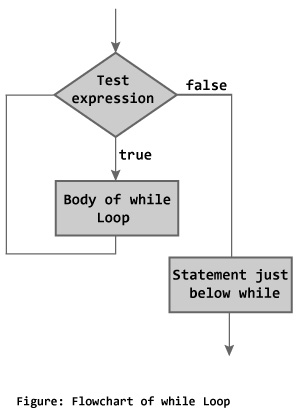
\includegraphics[width=.8\textwidth]{while.jpg}
\end{center}
\end{center}
\end{column}

\begin{column}{0.6\columnwidth}
\begin{block}{Ejemplo}
\begin{verbatim}
num = 1

while num <= 5:
  print(num)
  num = num + 1
\end{verbatim}
\scriptsize
\begin{verbatim}
1
2
3
4
5
\end{verbatim}
\end{block}
\end{column}
\end{columns}


\begin{block}{Bucles while}
Ejecuta el código tabulado mientras se cumpla la condición.
\end{block}
\end{frame}

\begin{frame}[fragile,label={sec:org55bb2cc}]{Tipos de bucle: for}
 \begin{columns}
\begin{column}{0.5\columnwidth}
\begin{exampleblock}{Ejemplo}
\begin{verbatim}
lista = ['a', 'b', 'c', 'd', 'e']

for num in lista:
  print(num)
\end{verbatim}
\end{exampleblock}
\end{column}
\begin{column}{0.5\columnwidth}
\begin{block}{Salida}
\scriptsize
\begin{verbatim}
a
b
c
d
e
\end{verbatim}
\end{block}
\end{column}
\end{columns}


\begin{block}{Bucles for}
\begin{description}
\item[{Formato}] for <variable> in <lista>:
bloque
\end{description}
\end{block}

\begin{block}{Significado}
\begin{itemize}
\item Por cada elemento de la lista:
\begin{itemize}
\item Asigna su valor en la variable.
\item Ejecuta el bloque de código tabulado.
\end{itemize}
\end{itemize}
\end{block}
\end{frame}


\begin{frame}[fragile,label={sec:org4d41cb9}]{Tipos de bucle: for}
 \begin{block}{Programador acostumbrado a otros lenguajes}
\begin{columns}
\begin{column}{0.4\columnwidth}
\begin{verbatim}
for i in range(0, len(lista)):
  print(lista[i])
\end{verbatim}
\end{column}

\begin{column}{0.5\columnwidth}
\begin{center}
\begin{center}

\includegraphics[width=.7\textwidth]{workinghard.jpg}
\end{center}
\end{center}
\end{column}
\end{columns}
\end{block}

\begin{block}{Programador \emph{pythonico}}
\begin{columns}
\begin{column}{0.5\columnwidth}
\begin{verbatim}
for elem in lista:
  print(elem)
\end{verbatim}
\end{column}

\begin{column}{0.3\columnwidth}
\begin{center}
\begin{center}

\includegraphics[width=.6\textwidth]{workingrelaxed.png}
\end{center}
\end{center}
\end{column}
\end{columns}
\end{block}
\end{frame}

\begin{frame}[fragile,label={sec:org6ac0d9c}]{Tipos de bucle: for}
 \begin{exampleblock}{¿Y si necesito el índice?}
\begin{verbatim}
for i, elem in enumerate(lista):
    print("El elemento", i, "vale", elem, "==", lista[i])
\end{verbatim}
\scriptsize
\begin{verbatim}
El elemento 0 vale 1 == 1
El elemento 1 vale 2 == 2
El elemento 2 vale 3 == 3
El elemento 3 vale 4 == 4
El elemento 4 vale 5 == 5
El elemento 5 vale 6 == 6
\end{verbatim}
\end{exampleblock}

\begin{block}{Función enumerate}
Recibe una lista, devuelve además de cada elemento de la lista, la posición (empezando por cero).
\end{block}
\end{frame}

\begin{frame}[fragile,label={sec:org42c083c}]{Tipos de bucle: for}
 \begin{exampleblock}{¿Y si necesito recorrer varias listas a la vez?}
\begin{verbatim}
nombres = ['Daniel', 'Amalia', 'Carlos', 'Rosa']
pies = [43, 41, 44, 42]

# Option 1: estilo C
for i in range(len(nombres)):
    print("Usuario", nombres[i], "tiene pie", pies[i])
# Option 2: Recorrido con enumerate
for i, nombre in enumerate(nombres):
    print("Usuario", nombre, "tiene pie", pies[i])
# Option 3: uso de zip
for nombre, pie in zip(nombres, pies):
    print("Usuario", nombre, "tiene pie", pie)
\end{verbatim}

Recibe varias listas, devuelve cada elemento de todas.
\end{exampleblock}
\end{frame}

\begin{frame}[fragile,label={sec:org4af7306}]{Formato inline de for}
 \begin{block}{Notación más matemática}
\begin{verbatim}
lista = [1, 2, 3, 4, 5]
doble = [2*x for x in lista]
print(doble)
doble_par = [2*x for x in lista if x % 2 == 0]
print(doble_par)
\end{verbatim}
\scriptsize
\begin{verbatim}
[2, 4, 6, 8, 10]
[4, 8]
\end{verbatim}
\end{block}

\begin{block}{Formato}
\begin{itemize}
\item\relax [expresion \alert{for} variable \alert{in} lista]

\item\relax [expresion \alert{for} variable \alert{in} lista \alert{if} condicion]
\end{itemize}
\end{block}
\end{frame}


\begin{frame}[fragile,label={sec:org822a48a}]{Concepto de iterador}
 \begin{block}{Iterador:}
\begin{itemize}
\item Función que devuelve una serie de elementos.

\item Se usan en los bucles for.

\item Se generan los elementos en cada ejecución del bucle, ahorra memoria.
\end{itemize}
\end{block}

\begin{columns}
\begin{column}{0.5\columnwidth}
\begin{exampleblock}{Ejemplo: range()}
\begin{verbatim}
ran = range(3)
# No muestra la lista
print(ran)
# Se puede recorrer ahora
for x in ran:
  print(x)
# O directamente
for x in range(3):
  print(x)
\end{verbatim}
\end{exampleblock}
\end{column}
\begin{column}{0.5\columnwidth}
\begin{block}{Salida}
\scriptsize
\begin{verbatim}
range(0, 3)
0
1
2
0
1
2
\end{verbatim}
\end{block}
\end{column}
\end{columns}
\end{frame}

\begin{frame}[fragile,label={sec:org9784394}]{Otros iteradores}
 \begin{block}{Métodos iteradores clásicos}
\begin{description}
\item[{map}] Aplica una función a cada elemento de una lista(secuencia).

\item[{filter}] Filtra los elementos de una lista.
\end{description}
\end{block}

\begin{columns}[t]
\begin{column}{0.5\columnwidth}
\begin{exampleblock}{Ejemplo}
\begin{verbatim}
pares = filter(espar, lista)

for x in pares:
  print(x)
\end{verbatim}
\end{exampleblock}
\end{column}
\begin{column}{0.5\columnwidth}
\begin{exampleblock}{espar}
\begin{verbatim}
def espar(x):
    return x % 2 == 0
\end{verbatim}
\scriptsize
\end{exampleblock}

\begin{block}{Salida}
\scriptsize
\begin{verbatim}
2
4
6
\end{verbatim}
\end{block}
\end{column}
\end{columns}
\end{frame}

\begin{frame}[fragile,label={sec:org8f68024}]{Posibles problemas con iteradores}
 \begin{columns}
\begin{column}{1.0\columnwidth}
\begin{alertblock}{Range es seguro}
\begin{itemize}
\item Otros métodos: map, filter, \ldots{} no lo son.

\item Eso implica que sólo se pueden ejecutar una vez.
\end{itemize}
\end{alertblock}
\end{column}
\end{columns}

\begin{columns}[t]
\begin{column}{0.5\columnwidth}
\begin{exampleblock}{Ejemplo}
\begin{verbatim}
pares = filter(espar, lista)
print("Primera vez")

for x in pares:
  print(x)

print("Repetimos")

for x in pares:
  print(x)
\end{verbatim}
\end{exampleblock}
\end{column}
\begin{column}{0.5\columnwidth}
\begin{block}{Salida}
\scriptsize
\begin{verbatim}
Primera vez
2
4
6
Repetimos
\end{verbatim}
\end{block}

\begin{exampleblock}{Posible solución}
\begin{verbatim}
pares = list(pares)
\end{verbatim}
\end{exampleblock}
\end{column}
\end{columns}
\end{frame}

\section{Funciones y clases}
\label{sec:org6b306ca}

\begin{frame}[fragile,label={sec:org96ac929}]{Funciones}
 \begin{block}{Funciones}
\begin{itemize}
\item Permiten no repetir el mismo código una y otra vez.

\item Se hace una única vez y se repite.
\end{itemize}
\end{block}

\begin{columns}
\begin{column}{0.5\columnwidth}
\begin{exampleblock}{Ejemplo}
\begin{verbatim}
def suma(lista):
  sum = 0

  for item in lista:
    sum += item

  return sum

print(suma([1, 3, 5]))
# Suma de 10 a 20
print(suma(range(10, 21)))
# Suma una sublista
lista = range(1, 101)
print(suma(lista[20:31]))
\end{verbatim}
\end{exampleblock}
\end{column}

\begin{column}{0.5\columnwidth}
\begin{block}{Salida}
\scriptsize
\begin{verbatim}
9
165
286
\end{verbatim}
\end{block}
\end{column}
\end{columns}
\end{frame}

\begin{frame}[fragile,label={sec:orgc8c690e}]{Sintaxis de las funciones}
 \begin{block}{Formato:}
\begin{verbatim}
def nombreFuncion(parametros):
  # Codigo
  # return salida
\end{verbatim}
\end{block}

\begin{block}{Bloque}
La tabulación limita el código dentro de la función.
\end{block}

\begin{block}{Estructura}
\begin{itemize}
\item La función puede recibir parámetros.

\item Puede devolver un valor mediante return, pero no es obligatorio.
\end{itemize}
\end{block}
\end{frame}

\begin{frame}[fragile,label={sec:org4271747}]{Ejemplo de funciones}
 \begin{block}{Máximo y mínimo}
\begin{verbatim}
def mymax(value1, value2):
    if value1 >= value2:
	return value1
    else:
	return value2

print(mymax(3, 5))
print(mymax(4, 2))
print(mymax(0, -2))
\end{verbatim}
\scriptsize
\begin{verbatim}
5
4
0
\end{verbatim}
\end{block}
\end{frame}

\begin{frame}[fragile,label={sec:org8438349}]{Funciones que devuelven valores}
 \begin{block}{Funciones}
Las más comunes son las que devuelven (\emph{return algo}). 
\end{block}

\begin{exampleblock}{Función que devuelve}
\begin{verbatim}
def add_vector(vector1, vector2):
    result = []

    for item1, item2 in zip(vector1, vector2):
	result.append(item1+item2)

    return result


print(add_vector([1, 2, 3], [4, 2, 3]))
\end{verbatim}
\scriptsize
\begin{verbatim}
[5, 4, 6]
\end{verbatim}
\end{exampleblock}
\end{frame}

\begin{frame}[fragile,label={sec:org847a425}]{Funciones que no devuelven valores}
 \begin{exampleblock}{Función que no devuelve}
\begin{verbatim}
def add_vector(vector1, vector2, result):
    result.clear()

    for item1, item2 in zip(vector1, vector2):
	result.append(item1+item2)

result = []
print("Imprimimos lo que devuelve la funcion")
print(add_vector([1, 2, 3], [4, 2, 3], result))
print("Ahora la variable de salida")
print(result)
\end{verbatim}
\scriptsize
\begin{verbatim}
Imprimimos lo que devuelve la funcion
None
Ahora la variable de salida
[5, 4, 6]
\end{verbatim}
\end{exampleblock}
\end{frame}


\begin{frame}[fragile,label={sec:orgaa4dfdc}]{Paso de parámetros}
 \begin{columns}
\begin{column}{0.5\columnwidth}
\begin{exampleblock}{Ejemplo con un entero}
\begin{verbatim}
def fun1(param):
    print(param)
    param = 4
    print(param)

variable = 3
fun1(variable)
print(variable)
\end{verbatim}
\scriptsize
\begin{verbatim}
3
4
3
\end{verbatim}
\end{exampleblock}
\end{column}

\begin{column}{0.5\columnwidth}
\begin{exampleblock}{Ejemplo con lista}
\begin{verbatim}
def fun2(param):
    print(param)
    param.clear()
    print(param)

variable = [3, 5, 7, 10]
fun2(variable)
print(variable)
\end{verbatim}
\scriptsize
\begin{verbatim}
[3, 5, 7, 10]
[]
[]
\end{verbatim}
\end{exampleblock}
\end{column}
\end{columns}

\begin{block}{Diferencia}
\begin{itemize}
\item El parámetro \emph{name} apunta al mismo dato que la variable que se pasa en la
llamada (\emph{variable}).

\item Cuando hace "name = \ldots{}" se le asigna un valor diferente, ya no son iguales.
\end{itemize}
\end{block}
\end{frame}

\begin{frame}[fragile,label={sec:orgb21b8f3}]{Parámetros opcionales}
 \begin{block}{Parámetros opcionales}
\begin{itemize}
\item Las funciones pueden tener parámetros por defecto.
\end{itemize}

\begin{verbatim}
def increm(value, increm=10):
    return value+increm

print(increm(3, 2))
print(increm(3, 10))
print(increm(3))
\end{verbatim}
\scriptsize
\begin{verbatim}
5
13
13
\end{verbatim}
\end{block}

\begin{block}{Posición de los parámetros por defecto}
\begin{itemize}
\item Deben aparecer al final.

\item Si no fuese así, no quedaría claro cómo interpretarlo si hay varias.
\end{itemize}
\end{block}
\end{frame}

\begin{frame}[fragile,label={sec:orgd0e0c59}]{Parámetros con nombre}
 \begin{block}{Parámetros con nombre}
No es necesario poner los parámetros en orden si se sabe su nombre.
\end{block}

\begin{columns}
\begin{column}{0.7\columnwidth}
\begin{exampleblock}{Ejemplo: copia de vector}
\begin{verbatim}
def mycopyvec(source, dest):
    dest.clear()

    # or dest.extend(source)
    for elem in source:
	dest.append(elem)

list1, list2 = [3, 4, 5], [2, 9, 7]
mycopyvec(list1, list2)
print("Lista1: ", list1)
print("Lista2: ", list2)
list1, list2 = [3, 4, 5], [2, 9, 7]
mycopyvec(dest=list1, source=list2)
print("Lista1: ", list1)
print("Lista2: ", list2)
\end{verbatim}
\end{exampleblock}
\end{column}
\begin{column}{0.3\columnwidth}
\begin{block}{Salida}
\scriptsize
\begin{verbatim}
Lista1:  [3, 4, 5]
Lista2:  [3, 4, 5]
Lista1:  [2, 9, 7]
Lista2:  [2, 9, 7]
\end{verbatim}
\end{block}
\end{column}
\end{columns}
\end{frame}



\section{Clases}
\label{sec:orge4c374b}

\begin{frame}[fragile,label={sec:orge0b9449}]{Clases}
 \begin{block}{Concepto de clases}
\begin{itemize}
\item En ciertos dominios requieren cierta información (Board).

\item Se realiza una serie de operaciones con la información.

\item Por comodidad se puede agrupar juntas.
\end{itemize}
\end{block}

\begin{exampleblock}{Si tenemos esto}
\begin{verbatim}
x = ...
y = ...
draw_board_battleship(x, y, size, fname_background, ...)
x += 1
draw_board_battleship(x, y, size, fname_background, ...)
\end{verbatim}
\end{exampleblock}

\begin{alertblock}{Errores}
\begin{itemize}
\item Para un simple concepto puede haber muchas variables.

\item Las funciones requieren muchos parámetros.
\end{itemize}
\end{alertblock}
\end{frame}

\begin{frame}[fragile,label={sec:org4e59c7f}]{Clases}
 \begin{block}{Es la forma que Python agrupa información}
\begin{itemize}
\item Agrupa variables y funciones sobre dichos datos.

\item Una instancia de la clase (variable) guarda esos datos como atributos.

\item No es necesario pasarle los datos, lo recoge de la variable.
\end{itemize}
\end{block}

\begin{exampleblock}{Ejemplo}
\begin{verbatim}
board = Board(x, y, size)
board.setBackground(fname_background)
board.draw()
board.move(inc_x=1)
board.draw()
\end{verbatim}
\end{exampleblock}
\end{frame}

\begin{frame}[label={sec:org48b2088}]{Clases}
\begin{block}{Python posee clases}
\begin{itemize}
\item Python tiene \alert{clases} como C++ o Java.

\item No posee estructuras.

\item No exige su uso como Java.

\item Se combina con enfoque estructural cuando conviene.
\end{itemize}
\end{block}

\begin{block}{Modelo de clases de Python}
\begin{itemize}
\item Ofrece la misma funcionalidad que otros.

\item Tiene sus particulares.

\begin{itemize}
\item No restricción de permisos.

\item Convenios de nomenclatura.

\item Propiedades.

\item Métodos especiales: str, init, \ldots{}
\end{itemize}
\end{itemize}
\end{block}
\end{frame}

\begin{frame}[fragile,label={sec:orgb63033a}]{Lo vemos por comparación}
 \begin{block}{Java}
\begin{verbatim}
public class Point {
    private int xCoord;
    private int yCoord;

    public Point() {
	xCoord = yCoord = 0;
    }
    public Point( int x, int y ) {
	xCoord = x;
	yCoord = y;
    }
    public String toString() {
	return "(" + xCoord + ", " + yCoord + ")";
    }
    public int getX() { return xCoord; }
    public int getY() { return yCoord; }
    public void shift( int xInc, int yInc ) {
	xCoord = xCoord + xInc;
	yCoord = yCoord + yInc;
    }
}
\end{verbatim}
\end{block}
\end{frame}

\begin{frame}[fragile,label={sec:orge054e0e}]{Lo vemos por comparación}
 \begin{block}{C++}
\begin{verbatim}
class Point {
private:
      int xCoord;
      int yCoord;

public:
      Point() {
	xCoord = yCoord = 0;
      }
      Point(int x, int y) {
	xCoord = x;
	yCoord = y;
      }
      int getX() { return xCoord; }
      int getY() { return yCoord; }

      void shift( int xInc, int yInc ) {
	xCoord = xCoord + xInc;
	yCoord = yCoord + yInc;
      }
};
\end{verbatim}
\end{block}
\end{frame}


\begin{frame}[fragile,label={sec:orgb6ba49b}]{Lo vemos por comparación}
 \begin{block}{Python}
\begin{verbatim}
class Point:

   def __init__(self, x = 0, y = 0):
      self.xCoord = x
      self.yCoord = y

   def __str__(self):
      return "({},{})".format(self.xCoord, self.yCoord)

   def getX(self):
      return self.xCoord

   def getY(self):
      return self.yCoord

   def shift(self, xInc, yInc):
      self.xCoord += xInc
      self.yCoord += yInc
\end{verbatim}
\end{block}
\end{frame}

\begin{frame}[label={sec:org0a6f7e9}]{Peculiaridades de clases}
\begin{block}{No límites de acceso}
\begin{itemize}
\item No hay límites de acceso.

\item Convenio: si empieza por "\_" no es público, no se debe acceder.
\end{itemize}
\end{block}

\begin{block}{Definir atributos}
\begin{itemize}
\item No sección especial.

\item Se hace con \alert{self.variable = \ldots{}} en el constructor.
\end{itemize}
\end{block}

\begin{block}{Métodos especiales:}
\begin{description}
\item[{\_\_init\_\_}] Constructor.

\item[{\_\_str\_\_}] Método para mostrar valores (conversión a cadena, \ldots{}).
\end{description}
\end{block}
\end{frame}

\begin{frame}[fragile,label={sec:org61ab6eb}]{Métodos en las clases}
 \begin{block}{Métodos:}
\begin{itemize}
\item Son funciones normales.

\item Recibe como primer parámetro el propio objeto (self).

\item El objeto self se usa para acceder a los atributos/métodos.

\item Todo método siempre tiene algún parámetro.
\end{itemize}
\end{block}

\begin{columns}
\begin{column}{0.6\columnwidth}
\begin{exampleblock}{Ejemplo de uso}
\begin{verbatim}
point = Point()
print(point)
point2 = Point(2, 3)
print(point2)
print(point2.getX())
point2.shift(1, -1)
print(point2)
# Acceso directo, no recomendado
point2.xCoord = 4
print(point2)
\end{verbatim}
\end{exampleblock}
\end{column}

\begin{column}{0.3\columnwidth}
\begin{block}{Salida}
\scriptsize
\begin{verbatim}
(0,0)
(2,3)
2
(3,2)
(4,2)
\end{verbatim}
\end{block}
\end{column}
\end{columns}
\end{frame}



\begin{frame}[fragile,label={sec:org037767f}]{Herencia}
 \begin{block}{Clase base}
\begin{verbatim}
class Polygon:
    def __init__(self, no_of_sides):
	self.n = no_of_sides
	self.sides = [Point(0,0) for i in range(self.n)]

    def setPoint(self, i, x, y):
	assert i >= 0 and i < self.n
	self.sides[i] = Point(x, y)

    def __str__(self):
	return ", ".join([str(t) for t in self.sides])

a = Polygon(2)
a.setPoint(0, x=1, y=2)
a.setPoint(1, x=1, y=1)
print(a)
\end{verbatim}
\scriptsize
\begin{verbatim}
(1,2), (1,1)
\end{verbatim}
\end{block}
\end{frame}

\begin{frame}[fragile,label={sec:org54db9c3}]{Herencia}
 \begin{block}{Clase heredada}
\begin{verbatim}
def copy(point, incX=0, incY=0):
    return Point(point.getX()+incX, point.getY()+incY)

class Rectangle(Polygon):
    def __init__(self, init, size):
	Polygon.__init__(self, 5)
	self.sides[0] = copy(init)
	self.sides[1] = copy(init, incY=size)
	self.sides[2] = copy(init, incX=size, incY=size)
	self.sides[3] = copy(init, incX=size)
	self.sides[4] = copy(init)

a = Rectangle(Point(0, 0), 3)
print(a)
a = Rectangle(Point(2, 2), 1)
print(a)
\end{verbatim}
\scriptsize
\begin{verbatim}
(0,0), (0,3), (3,3), (3,0), (0,0)
(2,2), (2,3), (3,3), (3,2), (2,2)
\end{verbatim}
\end{block}
\end{frame}

\begin{frame}[label={sec:org56de69e}]{Propiedades}
\begin{block}{Acceso a atributos}
\begin{itemize}
\item Python no suele usar métodos getX, setX.

\item Se puede acceder directamente a los métodos.

\item ¿Y si se desea limitar?
\end{itemize}
\end{block}

\begin{block}{Propiedades}
\begin{itemize}
\item Permite asignar método de asignación y consulta.

\item Es transparente.
\end{itemize}
\end{block}
\end{frame}

\begin{frame}[fragile,label={sec:orge4bc742}]{Propiedades}
 \begin{columns}
\begin{column}{0.75\columnwidth}
\begin{exampleblock}{Ejemplo}
\begin{verbatim}
class Temperature:
    def __init__(self, temperature):
	self.celsius = temperature

    @property
    def farenheit(self):
	return self.celsius*1.8+32

    @farenheit.setter
    def farenheit(self, value):
	self.celsius = (value-32)/1.8

temp = Temperature(30)
print(temp.celsius)
print(temp.farenheit)
temp.celsius = 40
print(temp.celsius)
print(temp.farenheit)
temp.farenheit = 100
print(temp.farenheit)
print(temp.celsius)
\end{verbatim}
\end{exampleblock}
\end{column}
\begin{column}{0.25\columnwidth}
\begin{block}{Salida}
\scriptsize
\begin{verbatim}
30
86.0
40
104.0
100.0
37.77777777777778
\end{verbatim}
\end{block}
\end{column}
\end{columns}
\end{frame}


\section{Librerías}
\label{sec:org4a5a62d}
\begin{frame}[label={sec:org6683006}]{Importando paquetes}
\begin{center}
\begin{center}

\includegraphics[width=.6\textwidth]{standing.png}
\end{center}
\end{center}



\begin{block}{No tienes que hacer todo el código}
\begin{itemize}
\item Reutilizar código externo, librerías/paquetes.

\begin{itemize}
\item Funciones o clases que podemos usar.
\end{itemize}
\end{itemize}
\end{block}
\end{frame}


\begin{frame}[label={sec:orgf192ac4}]{Estructurando el código}
\begin{block}{Dividiendo el programa}
\begin{itemize}
\item Podemos poner varias funciones en ficheros distintos. 

\begin{itemize}
\item Ej: utils.py, game.py, board.py, \ldots{}
\end{itemize}

\item Queremos usar esas funciones dentro de otros ficheros.
\end{itemize}
\end{block}

\begin{block}{Paquetes}
\begin{itemize}
\item Un paquete es un fichero (o varios) con funciones/clases.

\item Puede ser usado en otros ficheros.
\end{itemize}
\end{block}

\begin{block}{Distinto caso}
\begin{description}
\item[{Librería externa}] Nombre único del paquete, identifica la librería.

\item[{Fichero local}] El nombre del paquete es el del fichero (sin .py).
\end{description}
\end{block}
\end{frame}

\begin{frame}[fragile,label={sec:orgaa54847}]{Conflicto de nombres}
 \begin{block}{Conflicto de nombres}
\begin{itemize}
\item Una misma función puede existir en varios paquetes.
\end{itemize}
\end{block}


\begin{block}{Import}
\begin{verbatim}
import package
...
package.fun(...)
\end{verbatim}
\end{block}

\begin{columns}
\begin{column}{0.6\columnwidth}
\begin{exampleblock}{Sin usar import}
\begin{verbatim}
print(sqrt(9))
\end{verbatim}
\scriptsize
\begin{verbatim}
Traceback (most recent call last):
  File "<stdin>", line 1, in <module>
NameError: name 'sqrt' is not defined
\end{verbatim}
\end{exampleblock}
\end{column}

\begin{column}{0.4\columnwidth}
\begin{exampleblock}{Con import}
\begin{verbatim}
import math
print(math.sqrt(9))
\end{verbatim}
\scriptsize
\begin{verbatim}
3.0
\end{verbatim}
\end{exampleblock}
\end{column}
\end{columns}
\end{frame}

\begin{frame}[fragile,label={sec:org668547c}]{Otras opciones}
 \begin{block}{Indicar las funciones usadas de cada paquete}
from \emph{package} import \emph{fun1}, \emph{fun2}, \ldots{}, \emph{funN}
\end{block}

\begin{exampleblock}{Ejemplo}
\begin{verbatim}
from math import sqrt
print(sqrt(9))
\end{verbatim}
\end{exampleblock}

\begin{block}{¿Y si hay muchas funciones?}
\begin{itemize}
\item Podría ser mejor usar paquete. \pause \(\Rightarrow\) ¿Y si no me gusta?
\end{itemize}
\pause
\end{block}
\begin{columns}
\begin{column}{0.6\columnwidth}
\begin{exampleblock}{Uso de alias}
\begin{verbatim}
import numpy as np

a = np.zeros(5)
print(a)
\end{verbatim}
\end{exampleblock}
\end{column}

\begin{column}{0.3\columnwidth}
\begin{block}{Salida}
\scriptsize
\begin{verbatim}
[ 0.  0.  0.  0.  0.]
\end{verbatim}
\end{block}
\end{column}
\end{columns}
\end{frame}


\begin{frame}[fragile,label={sec:orgf0a196d}]{Ejemplo local}
 \begin{block}{Fichero utils.py}
\begin{verbatim}
def print_hello():
  print("Hola")

def print_adios():
  print("Adios")
\end{verbatim}
\end{block}

\begin{exampleblock}{Fichero main.py (mismo directorio)}
\begin{verbatim}
import utils

utils.print_hello()
print("Bla Bla Bla")
utils.print_adios()
\end{verbatim}
\scriptsize
\begin{verbatim}
Hola
Bla Bla Bla
Adios
\end{verbatim}
\end{exampleblock}
\end{frame}

\begin{frame}[fragile,label={sec:org088a19c}]{Programa main}
 \begin{block}{Al hacer import se ejecuta el fichero}
\begin{itemize}
\item No es adecuado poner código fuera de las funciones.

\item Es conveniente una función \alert{main}.
\end{itemize}
\end{block}

\begin{exampleblock}{Función main}
\begin{verbatim}
def main():
    print("Hola a todos")

if __name__ == "__main__":
    main()
\end{verbatim}
\scriptsize
\begin{verbatim}
Hola a todos
\end{verbatim}
\end{exampleblock}

\begin{block}{Comentarios}
\begin{itemize}
\item La función puede tener cualquier nombre.

\item Se garantiza que sólo se ejecuta como programa, no por un import.
\end{itemize}
\end{block}
\end{frame}

\begin{frame}[label={sec:org0e02e1f}]{Instalar paquetes}
\begin{center}
\begin{center}

\includegraphics[width=0.453\textwidth]{box_python.png}
\end{center}
\end{center}

\begin{block}{Instalación}
\begin{itemize}
\item Python permite instalar muy fácilmente paquetes.

\item Existe un repositorio oficial de paquetes: PyPI.

\item[{Pip}] programa para buscar/instalar/borrar paquetes (y sus dependencias).
\end{itemize}
\end{block}
\end{frame}

\begin{frame}[fragile,label={sec:org39086fd}]{Uso de Pip}
 \begin{block}{Buscar: search}
\begin{verbatim}
pip search cec2013lsgo
\end{verbatim}
\scriptsize
\begin{verbatim}
cec2013lsgo (2.1)  - Package for benchmark for the Real ...
                     Evolutionary Computation CEC'2013
  INSTALLED: 2.0
  LATEST:    2.1
\end{verbatim}
\end{block}

\begin{block}{Información: show}
\begin{verbatim}
pip show cec2013lsgo
\end{verbatim}
\scriptsize
\begin{verbatim}
Name: cec2013lsgo
Version: 2.0
Summary: Package for benchmark for the Real ...
Home-page: https://github.com/dmolina/cec2013lsgo
Author: Daniel Molina
Author-email: dmolina@decsai.ugr.es
License: GPL V3
Location: /mnt/home/daniel/anaconda3/lib/python3.6/site-packages/...
Requires: cython, numpy
\end{verbatim}
\end{block}
\end{frame}

\begin{frame}[fragile,label={sec:orgec4bf45}]{Uso de Pip}
 \begin{block}{Instalar: install}
\begin{verbatim}
pip install numpy
\end{verbatim}
\scriptsize
\begin{verbatim}
Requirement already satisfied: numpy in ...
\end{verbatim}
\end{block}

\begin{block}{Borrar: uninstall}
\begin{verbatim}
pip uninstall cec2013lsgo
\end{verbatim}
\scriptsize
\begin{verbatim}
Successfully uninstalled cec2013lsgo-2.0
\end{verbatim}
\end{block}
\end{frame}


\begin{frame}[fragile,label={sec:org09091ba}]{Uso de pip y permisos}
 \begin{block}{¿Y si no tengo permisos?}
Se puede instalar en el \$HOME del usuario con:

\begin{verbatim}
pip install numpy --user
\end{verbatim}
\end{block}

\begin{columns}
\begin{column}{0.8\columnwidth}
\begin{alertblock}{Aviso}
Es recomendable usarlo y no hacer "sudo pip".
\end{alertblock}
\end{column}
\end{columns}
\end{frame}


\begin{frame}[label={sec:orgb8d05a1}]{Cargando un módulo}
\begin{block}{Librerías y ejecutables}
\begin{itemize}
\item Hay librerías que ofrecen programas ejecutables.

\item También la librería puede contener una función main asociada.
\end{itemize}
\end{block}

\begin{block}{Cargando un módulo}
\begin{itemize}
\item Con la opción "-m" se puede cargar un módulo.
\end{itemize}
\end{block}
\end{frame}

\begin{frame}[fragile,label={sec:orgd75bd87}]{Ejemplo: Carga de módulo}
 \begin{block}{Detección estática}
\begin{verbatim}
python -m mypy check.py
\end{verbatim}
\end{block}


\begin{block}{Otro ejemplo: servidor web}
\begin{verbatim}
python3 -m http.server
\end{verbatim}
\scriptsize
Serving HTTP on 0.0.0.0 port 8000 (\url{http://0.0.0.0:8000/}) \ldots{}
127.0.0.1 - - [19/Apr/2018 18:57:45] "GET / HTTP/1.1" 200 -
\end{block}
\end{frame}

\begin{frame}[label={sec:orgcbb08a1}]{Conflicto entre paquetes}
\begin{block}{Posible situación}
\begin{itemize}
\item Paquete1 \(\Rightarrow\) v2.0 de Paquete4

\item Paquete3 \(\Rightarrow\) v3.0 de Paquete4
\end{itemize}
\end{block}

\begin{block}{¿Como se puede resolver?}
\begin{itemize}
\item Se puede instalar las librerías en directorios distintos.
\begin{itemize}
\item Paquete1 y v2.0 de Paquete4 en uno.
\item Paquete3 y v3.0 de Paquete4 en otro.
\end{itemize}

\item Activar el entorno que queremos (usar las librerías de un directorio u otro).

\item Así además si la librería incluye ejecutable lo tendremos configurado.
\end{itemize}
\end{block}
\end{frame}

\begin{frame}[label={sec:org84a097d}]{Herramientas de entornos}
\begin{block}{Conda}
\begin{itemize}
\item Específico de Anaconda.

\item No compatible con otros.
\end{itemize}
\end{block}

\begin{block}{pipenv}
\begin{itemize}
\item Muy reciente (1 año y poco).

\item Considerado el estándar.
\end{itemize}
\end{block}

\begin{block}{Otros (pyenv, venv)}
\begin{itemize}
\item Anteriores a pipenv.
\end{itemize}
\end{block}
\end{frame}

\begin{frame}[label={sec:org7c973e3}]{Conflicto de paquetes: uso de conda}
\begin{block}{conda}
\begin{description}
\item[{Ver los entornos}] conda env list. El actual está marcado con *.

\item[{Crear un entorno}] conda create -n \emph{nombre} [opciones].

\item[{Activar entorno}] source activate \emph{nombre}.

\item[{Desactivar entorno actual}] source deactivate.
\end{description}
\end{block}
\end{frame}

\begin{frame}[fragile,label={sec:org007d1fc}]{Ejemplo de uso de conda}
 \begin{block}{Lista}
\begin{verbatim}
conda env list
\end{verbatim}
\end{block}

\begin{block}{Salida}
\scriptsize
\begin{verbatim}
# conda environments:
#
base                  *  /mnt/home/daniel/anaconda3
IA                       /mnt/home/daniel/anaconda3/envs/IA
curso                    /mnt/home/daniel/anaconda3/envs/curso
wcci2018                 /mnt/home/daniel/anaconda3/envs/wcci2018
\end{verbatim}
\end{block}
\end{frame}

\begin{frame}[fragile,label={sec:orged9843e}]{Uso de entorno}
 \begin{exampleblock}{Configurar paquetes (se indica en la shell)}
\begin{verbatim}
daniel@ubuntu:~/working$ source activate IA
(IA) daniel@ubuntu:~/working$ pip install ...
(IA) daniel@ubuntu:~/working$ source deactivate
daniel@ubuntu:~/working$ 
\end{verbatim}
\end{exampleblock}

\begin{exampleblock}{Cargar programa usando el entorno (se indica en la shell)}
\begin{verbatim}
daniel@ubuntu:~/working$ source activate IA
(IA) daniel@ubuntu:~/working$ python ...
(IA) daniel@ubuntu:~/working$ source deactivate
daniel@ubuntu:~/working$ 
\end{verbatim}
\end{exampleblock}
\end{frame}

\begin{frame}[label={sec:orgfa304b6}]{Herramienta de entorno: pipenv}
\begin{center}
\href{https://vimeo.com/233134524}{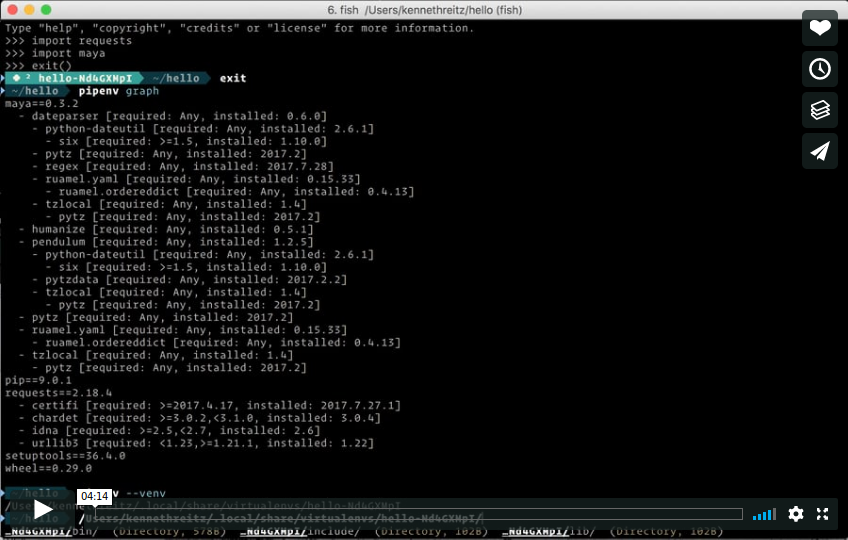
\includegraphics[width=\textwidth]{pipenv.png}}
\end{center}
\end{frame}


\section{Uso de ficheros}
\label{sec:org561d534}

\begin{frame}[label={sec:org24c7fa9}]{Uso de ficheros}
\begin{block}{Un programa no está solo en el sistema}
\begin{itemize}
\item Tiene que comunicarse.

\item La forma primordial es usando ficheros.
\end{itemize}
\end{block}

\begin{block}{Dos formas de interactuar}
\begin{itemize}
\item Leer y escribir ficheros.

\item Conocer la estructura de ficheros/directorios del ordenador.
\end{itemize}
\end{block}
\end{frame}

\begin{frame}[label={sec:org6985e46}]{Uso de ficheros con Python}
\begin{block}{Sentencia with}
\begin{itemize}
\item Uso de \alert{with} para abrir ficheros.

\item Permite agrupar el código y no preocuparse de cerrar fichero.
\end{itemize}
\end{block}

\begin{block}{Mayor sencillez}
\begin{itemize}
\item Alternativa librería os.path \(\Rightarrow\) libpath.

\item Uso de print para escribir en ficheros.
\end{itemize}
\end{block}
\end{frame}

\begin{frame}[fragile,label={sec:org4b207cb}]{Sentencia with}
 \begin{block}{Sentencia with}
\begin{itemize}
\item Uso de \alert{with} para abrir ficheros.

\item Permite agrupar el código y no preocuparse de cerrar fichero.
\end{itemize}
\end{block}

\begin{exampleblock}{Código}
\begin{verbatim}
# No es necesario cerrarlo, file es local para el bloque
with open("salida.txt", "w") as file:
    print("Hola a todos", file=file)
    print("Hasta luego", file=file)
\end{verbatim}
\end{exampleblock}

\begin{block}{¿Qué hace?}
\begin{enumerate}
\item Crea la variable \emph{file} asociada al nuevo fichero "salida.txt".

\item Escribe un mensaje usando la variable \emph{file}.

\item Al terminar el bloque el fichero se cierra.
\end{enumerate}
\end{block}
\end{frame}

\begin{frame}[fragile,label={sec:orgb643684}]{Cierre automático del fichero}
 \begin{block}{Ejemplo incorrecto}
\begin{verbatim}
# No es necesario cerrarlo, file es local para el bloque
with open("salida.txt", "w") as file:
    print("Hola a todos", file=file)

print("Otro mensaje", file=file)
\end{verbatim}
\end{block}

\begin{alertblock}{Da error}
\scriptsize
\begin{verbatim}
Traceback (most recent call last):
  File "<stdin>", line 1, in <module>
  File "/tmp/babel-1017136Z/python-10171jGE", line 5, in <module>
    print("Otro mensaje", file=file)
ValueError: I/O operation on closed file.
\end{verbatim}
\end{alertblock}
\end{frame}

\begin{frame}[fragile,label={sec:org3e9f57c}]{Modos de open}
 Puede contener como parámetro una cadena "\emph{modo}" o "\emph{modotipo}, en donde:

\begin{block}{Modos de fichero}
\begin{description}
\item[{r (por defecto)}] Abrirlo para leer, si no existe lanza excepción.

\item[{w}] Abrirlo para escribir, si existe lo borra antes.

\item[{a}] Abrirlo para escribir, si existe añade al final.
\end{description}
\end{block}

\begin{block}{Tipo de fichero}
\begin{description}
\item[{t (Por defecto)}] Fichero de texto.

\item[{b}] Fichero binario.
\end{description}
\end{block}

\begin{block}{Ejemplo}
\begin{verbatim}
open(fname, "r") # Abre para leer
open(fname, "wb") # Escribe fichero binario
open(fname, "a") # Concatena uno de texto
\end{verbatim}
\end{block}
\end{frame}

\begin{frame}[fragile,label={sec:org6416730}]{Escribiendo fichero binario}
 \begin{block}{Leyendo: read(longitud)}
\begin{verbatim}
with open("completo.pdf", "rb") as file:
    head = file.read(22)
    print(head)
    second = file.read(5)
    print(second)
\end{verbatim}
\scriptsize
\begin{verbatim}
b'%PDF-1.5\n%\xd0\xd4\xc5\xd8\n17 0 ob'
b'j\n<<\n'
\end{verbatim}
\end{block}

\begin{block}{Escribiendo: write(buffer)}
\begin{verbatim}
with open("completo.pdf", "rb") as finput:
    with open("copia.pdf", "wb") as foutput:

	buffer = finput.read(1024)

	while buffer:
	    second = foutput.write(buffer)
	    buffer = finput.read(1024)
\end{verbatim}
\scriptsize
\end{block}
\end{frame}

\begin{frame}[fragile,label={sec:org516a067}]{Fichero de texto: leer}
 \begin{block}{readline: Lee una línea}
\begin{verbatim}
with open("salida.txt") as file:
  line = file.readline()
  print("Linea 1:", line)
  print("Linea 1:", line.rstrip())
  line = file.readline()
  print("Linea 2:", line)
\end{verbatim}
\scriptsize
\begin{verbatim}
Linea 1: Hola a todos

Linea 1: Hola a todos
Linea 2: Hasta luego
\end{verbatim}
\end{block}

\begin{block}{readlines: Lee todo el fichero de golpe}
\begin{verbatim}
with open("salida.txt") as file:
  lines = file.readlines()
  print("Lineas:", lines)
\end{verbatim}
\scriptsize
\begin{verbatim}
Lineas: ['Hola a todos\n', 'Hasta luego\n']
\end{verbatim}
\end{block}
\end{frame}

\begin{frame}[fragile,label={sec:org67ef8e9}]{Fichero de texto: iteración}
 \begin{block}{Iterar un fichero da las líneas}
\begin{verbatim}
with open("salida.txt") as file:
    for line in file:
	print(line)
\end{verbatim}
\scriptsize
\begin{verbatim}
Hola a todos

Hasta luego
\end{verbatim}
\end{block}

\begin{alertblock}{Cuidado con los retornos de carro}
\begin{verbatim}
with open("salida.txt") as file:
    for line in file:
	print(line.rstrip())
\end{verbatim}
\scriptsize
\begin{verbatim}
Hola a todos
Hasta luego
\end{verbatim}
\end{alertblock}
\end{frame}

\begin{frame}[fragile,label={sec:org9b3565e}]{Fichero de texto: escribir}
 \begin{block}{Usar write}
\begin{verbatim}
with open("salida.txt", "a") as fout:
    fout.write("Nueva linea\n")
\end{verbatim}
\scriptsize
\end{block}

\begin{block}{Uso de print}
\begin{itemize}
\item print puede escribir.
\end{itemize}

\begin{verbatim}
with open("salida.txt", "a") as fout:
    print("Otra linea", file=fout)
\end{verbatim}
\scriptsize
\end{block}
\end{frame}

\begin{frame}[label={sec:org4c10693}]{Trabajando con ficheros}
\begin{block}{No todo es with}
\begin{itemize}
\item No todo es escribir y leer ficheros
\end{itemize}
\end{block}

\begin{block}{Es necesario trabajar con ficheros}
\begin{itemize}
\item Listas ficheros.

\item Gestionar directorios.

\item Gestionar ficheros: borrar, renombrar, \ldots{}
\end{itemize}
\end{block}
\end{frame}

\begin{frame}[fragile,label={sec:orga64b8b8}]{Trabajando con ficheros}
 \begin{block}{os.system}
Permite ejecutar una orden del SO.
\end{block}

\begin{exampleblock}{Ejemplo con system}
\begin{verbatim}
import os
os.system("ls *.pdf")
\end{verbatim}
\scriptsize
\begin{verbatim}
completo.pdf  copia.pdf  usage.pdf
\end{verbatim}
\end{exampleblock}

\begin{alertblock}{Cuidado}
\begin{itemize}
\item \alert{os.system} no es \emph{portable} entre SOs.

\item Hay otras alternativas \emph{portables}.
\end{itemize}
\end{alertblock}
\end{frame}

\begin{frame}[fragile,label={sec:org2d5e356}]{Listar ficheros}
 \begin{block}{Listar}
\begin{description}
\item[{glob(pattern)}] Permite buscar ficheros usando *.

\item[{os.listdir(dir)}] Lista un directorio.
\end{description}
\end{block}

\begin{exampleblock}{Ejemplo}
\begin{verbatim}
import os, glob
pdfs = glob.glob("*.pdf")
pdfs2 = [dir for dir in os.listdir('.') if ".pdf" in dir]
print(pdfs)
print(pdfs2)
\end{verbatim}
\scriptsize
\begin{verbatim}
['copia.pdf', 'completo.pdf', 'usage.pdf']
['copia.pdf', 'completo.pdf', 'usage.pdf']
\end{verbatim}
\end{exampleblock}
\end{frame}

\begin{frame}[label={sec:orge52fffb}]{Trabajar con directorios}
\begin{block}{Editar directorios}
\begin{description}
\item[{os.mkdir(dir)}] Crear directorio.
\item[{os.chdir(dir)}] Cambiar de directorio.
\item[{os.curdir}] Directorio actual.
\item[{os.rmdir(dir)}] Borrar directorio.
\end{description}
\end{block}

\begin{block}{Editar ficheros}
\begin{description}
\item[{os.remove(fname)}] Borra fichero.
\item[{os.rename(fold, fnew)}] Cambiar el nombre de directorio.
\item[{shutil.copy(origen, destino)}] Copiar fichero o directorio.
\item[{shutil.rmtree(dir)}] Borra directorio (cuidado).
\end{description}
\end{block}
\end{frame}

\begin{frame}[fragile,label={sec:orgf63eb48}]{Librería pathlib}
 \begin{block}{Nuevo interfaz}
\begin{itemize}
\item Clase Path con muchos métodos.

\item Totalmente independiente del SO.
\end{itemize}
\end{block}

\begin{block}{Ejemplo}
\begin{verbatim}
import pathlib
dir = pathlib.Path('.')
files = [file.name for file in dir.glob("*.pdf")]
print(files)
\end{verbatim}
\scriptsize
\begin{verbatim}
['copia.pdf', 'completo.pdf', 'usage.pdf']
\end{verbatim}
\end{block}
\end{frame}

\begin{frame}[fragile,label={sec:org00a9aba}]{Acceso a ficheros desde libpath}
 \begin{block}{Ejemplo}
\begin{verbatim}

from pathlib import Path
dir = Path('.')
file = dir / "usage.pdf"

if file.exists():
  if file.is_dir():
    print(file.name, "es un directorio")
  else:
    print(file.name, "es un fichero")
    file.
\end{verbatim}
\scriptsize
\begin{verbatim}
usage.pdf es un fichero
\end{verbatim}
\end{block}
\end{frame}

\begin{frame}[fragile,label={sec:orgd06b5e3}]{Trabajando con libpath}
 \begin{block}{Cambiando jpg -> jpeg}
\begin{verbatim}
import pathlib
dir = pathlib.Path('.')
subdirs = [x for x in dir.iterdir() if x.is_dir()]
print(subdirs)

dir = Path('.') / 'borra'
print(dir.resolve())


if dir.exists():
    files = list(dir.glob("*.jpeg"))

    for file in files:
	new_fname = str(file).replace(".jpeg", ".jpg")
	file.rename(new_fname)
\end{verbatim}
\scriptsize
\begin{verbatim}
[PosixPath('auto'), PosixPath('borra'), PosixPath('notebooks')]
/mnt/home/daniel/working/docencia/ceuta/201718/curso_python/slides/borra
\end{verbatim}
\end{block}
\end{frame}

\section{}
\label{sec:org7d57cb8}
\begin{frame}[label={sec:orgd9d09e3}]{License}
\begin{block}{Se puede obtener este curso (y otro material) de}
\begin{center}
\url{https://github.com/dmolina/curso\_python}
\end{center}
\end{block}

\begin{block}{Material disponible bajo licencia}
\href{http://creativecommons.org/licenses/by-sa/4.0/}{Creative Commons Attribution-ShareAlike 4.0 International License}
\end{block}

\begin{exampleblock}{Licencia}
\begin{center}
%\ccbysa
\end{center}
\end{exampleblock}
\end{frame}
\end{document}